%% LyX 2.5.2 created this file.  For more info, see https://www.lyx.org/.
%% Do not edit unless you really know what you are doing.
\documentclass[journal,article,submit,moreauthors]{Definitions/mdpi}
\usepackage{textcomp}
\usepackage[utf8]{inputenc}
\synctex=-1
\usepackage{float}
\usepackage{url}
\usepackage{amstext}
\usepackage{graphicx}

\makeatletter

%%%%%%%%%%%%%%%%%%%%%%%%%%%%%% LyX specific LaTeX commands.

\Title{Enhancing Rule Construction in Grammatical Evolution with Advanced
Crossover Techniques}

\Author{\textsubscript{\textsuperscript{}}Ioannis G. Tsoulos$^{1*}$, Georgios
Georgoulas$^{2}$ and Vasileios Charilogis$^{3}$}


\address{$^{1}\quad$Department of Informatics and Telecommunications. University
of Ioannina, Greece; itsoulos@uoi.gr\\
$^{2}$\quad{}Department of Mechanical Engineering and Aeronautics,
University of Patras, Panepistimioupoli Patron, Rio 26504, Greece;
georgoul@gmail.com\\
$^{3}\quad$Department of Informatics and Telecommunications. University
of Ioannina, Greece; charilog@uoi.gr}


\corres{Correspondence: itsoulos@uoi.gr}


\abstract{Many real-world problems can be formulated as classification tasks
in machine learning and addressed using a wide range of advanced algorithms
developed for this purpose. Among these approaches, methods based
on Grammatical Evolution (GE) can also be employed, such as GenClass,
a technique designed to automatically construct classification rules.
Although GenClass has been successfully applied to a variety of classification
problems, its evolutionary search process may suffer from limitations
such as entrapment in local minima of the error function and premature
convergence, which can prevent the method from discovering high-quality
classification rules. The present work proposes an enhanced version
of GenClass through the introduction of advanced crossover techniques
operating on the integer-valued chromosomes employed by the method,
with the aim of achieving a significant reduction in classification
error. The proposed crossover operators follow two different strategies.
Some of them are purely stochastic, introducing greater diversity
into the evolutionary search, whereas others exploit information already
generated during the Grammatical Evolution process to perform targeted
exchanges of genetic material between chromosomes. In this way, the
latter operators attempt to guide the evolutionary search toward more
promising regions of the search space while preserving useful information
discovered during previous generations. The proposed techniques were
evaluated on a diverse collection of real-world classification datasets,
including several problems characterized by a large number of patterns
and/or a large number of classes. The experimental results demonstrate
that the proposed crossover strategies can substantially improve the
performance of the original method, leading to a noticeable reduction
in classification error across a wide range of classification problems.}


\keyword{Grammatical Evolution; Classification; Crossover Operators; Evolutionary
Algorithms; Machine Learning.}

\DeclareTextSymbolDefault{\textquotedbl}{T1}
%% Because html converters don't know tabularnewline
\providecommand{\tabularnewline}{\\}

%%%%%%%%%%%%%%%%%%%%%%%%%%%%%% User specified LaTeX commands.
%  LaTeX support: latex@mdpi.com
%  For support, please attach all files needed for compiling as well as the log file, and specify your operating system, LaTeX version, and LaTeX editor.
%=================================================================
%\documentclass[journal,article,submit,moreauthors,unicode]{Definitions/mdpi} % For some letters Palatino lacks
%\documentclass[preprints,article,submit,moreauthors]{Definitions/mdpi} 
%\documentclass[preprints,article,submit,moreauthors,unicode]{Definitions/mdpi} 
% For posting an early version of this manuscript as a preprint, you may use "preprints" as the journal. Changing "submit" to "accept" before posting will remove line numbers.

%--------------------
% Class Options:
%--------------------
%----------
% journal
%----------
% Choose between the following MDPI journals:

% Below journals will use APA reference format:
% admsci, aieduc, behavsci, businesses, econometrics, economies, education, ejihpe, famsci, fclam, games, humans, ijcs, ijfs, investment, joi, jintelligence, journalmedia, jrfm, jsam, languages, opermanag, peacestud, pmh, psycholint, publications, sciedu, tourismhosp, xmanagement, youth

% Below journals will use Chicago reference format:
% arts, genealogy, histories, humanities, laws, literature, religions, risks, socsci

% Below journals will use ACS reference format:
% accountaudit, acn, acoustics, actuators, addictions, addictprev, adhesives, adolescents, aee, aerobiology, aeronautics, aerospace, agriculture, agriengineering, agrochemicals, agronomy, ai, aiagents, aichem, aieng, aimater, aimed, aipa, air, aisens, aisoc, algorithms, allergies, alloys, amh, analog, analytica, analytics, anatomia, anesthres, animals, antibiotics, antibodies, antioxidants, applbiosci, appliedchem, appliedmath, appliedphys, applmech, applmicrobiol, applnano, applsci, aps, aquacj, archaeolstud, architecture, arm, arthropoda, asc, asd, asi, astronautics, astronomy, atmosphere, atoms, audiolres, automation, axioms, bacteria, batteries, bcrc, bdcc, beverages, bioactives, biochem, bioengineering, biologics, biology, biomass, biomechanics, biomed, biomedicines, biomedinformatics, biomimetics, biomolecules, biophysica, bioresourbioprod, biosensors, biosphere, biotech, birds, blockchains, bloods, blsf, brainsci, breath, buildings, cancers, carbon, cardio, cardiogenetics, cardiovascmed, catalysts, cells, ceramics, challenges, chemeco, chemengineering, chemistry, chemosensors, chemproc, children, chips, cimb, civileng, cleantechnol, climate, clinbioenerg, clinpract, clockssleep, cmd, cmtr, coasts, coatings, colloids, colorants, commodities, complexities, complications, compounds, computation, computers, condensedmatter, conservation, constrmater, cosmetics, covid, crops, cryo, cryptography, crystals, csmf, ctn, culture, curroncol, cyber, dairy, data, ddc, dentistry, dermato, dermatopathology, designs, devices, dgg, dhi, diabetology, diagnostics, dietetics, digital, disabilities, diseases, diversity, dna, drones, drugreact, drylands, dynamics, earth, ebj, ece, ecm, ecologies, edm, eesp, electricity, electrochem, electronicmat, electronics, embodiedintell, encyclopedia, endocrines, energies, eng, engproc, entomology, entropy, environments, environremediat, enzymology, epidemiologia, epigenomes, epilepsy, esa, est, fermentation, fibers, fintech, fire, fishes, fluids, foodeng, foods, forecasting, forensicsci, forests, fossstud, foundations, fractalfract, freshwater, fuels, future, futureinternet, futurepharmacol, futurephys, futuretransp, galaxies, gases, gastroent, gastrointestdisord, gastronomy, gels, genes, geochem, geographies, geohazards, geomatics, geometry, geosciences, geotechnics, geriatrics, germs, glacies, grainsci, grasses, green, greenhealth, gucdd, gynecolcancer, hardware, hazardousmatters, healthcare, healthcmater, hearts, hemato, hematolrep, hep, heritage, higheredu, highthroughput, horticulturae, hospitals, humanoids, hydrobiology, hydrogen, hydrology, hydrometeorology, hydropower, hygiene, idr, iic, ijem, ijerph, ijgi, ijmd, ijms, ijns, ijom, ijp, ijpb, ijt, ijtm, ijtpp, ijtst, ime, immuno, industries, inflammj, informatics, information, infrastructures, inorganics, insects, instruments, inventions, iot, iron, j, jaestheticmed, jal, japma, jcdd, jcm, jcp, jcrm, jcs, jcto, jdad, jdb, jdcp, jdream, jemr, jeta, jfb, jfmk, jfth, jgbg, jgg, jimaging, jlpea, jmahp, jmmp, jmms, jmp, jmse, jne, jnt, jof, joitmc, joma, jop, joptm, jor, jox, jpbi, jphytomed, jpm, jsan, jtaer, jvd, jzbg, kidneydial, kinasesphosphatases, knowledge, labmed, laboratories, lam, land, langtechnol, lasers, legumes, life, lights, limnolrev, lipidology, liquids, livers, logics, logistics, lubricants, lymphatics, machines, macromol, magnetism, magnetochemistry, make, marinedrugs, maritime, materials, materproc, mathematics, mca, mcb, measurements, meb, medicina, medicines, medsci, membranes, merits, metabolites, metals, metamaterialsadv, meteorology, methane, metrics, metrology, micro, microarrays, microbiolres, microelectronics, micromachines, microorganisms, microplastics, microwave, minerals, mining, mmphys, modelling, molbank, molecules, mollusca, mps, msf, mti, multimedia, muscles, mutation, nanoenergyadv, nanomanufacturing, nanomaterials, ncrna, ndt, network, neuroglia, neuroimaging, neurolint, neurosci, nitrogen, notspecified, nursrep, nutraceuticals, nutrients, obesities, occuphealth, oceans, ohbm, onco, optics, optoelectronics, oral, organics, organoids, osteology, oxygen, pandemics, parasites, parasitologia, particles, pathogens, pathophysiology, pediatrrep, pets, pharmaceuticals, pharmaceutics, pharmacoepidemiology, pharmacy, phc, philosophies, photochem, photonics, photovoltaics, phycology, physchem, physics, physiologia, plants, plasma, platforms, pnr, pollutants, polymers, polysaccharides, populations, poultry, powders, precision, precisoncol, preprints, prevhealthc, proceedings, processes, prosthesis, proteomes, psf, psychiatryint, psychoactives, purification, quantumrep, quaternary, qubs, radiation, rareearths, rdt, reactions, realestate, receptors, recycling, regeneration, remotesensing, reports, reprodmed, resources, rheumato, rjpm, robotics, rsee, ruminants, safety, sanpp, sca, sci, scipharm, sclerosis, seeds, sensors, senssyst, separations, sexes, shi, signals, sinusitis, siuj, skins, smartcities, smartfish, smartgrids, sna, societies, software, soilsystems, solar, solids, spectroscj, sports, standards, stats, std, stratsediment, stresses, strokerep, superintelligence, surfaces, surgeries, susagric, suschem, sustainability, sustainfoods, sustainpackag, symmetry, synbio, systems, tae, targets, taxonomy, technologies, telecom, test, textiles, thalassrep, therapeutics, thermo, timespace, tomography, toxics, toxins, tph, transplantology, transportation, traumacare, traumas, tri, tropicalmed, universe, urbansci, uro, vaccines, vehicles, venereology, vetsci, vibration, virtualworlds, viruses, vision, waste, water, welding, wem, wevj, wild, wind, women, world, zoonoticdis

%---------
% article
%---------
% The default type of manuscript is "article", but can be replaced by: 
% abstract, addendum, article, benchmark, book, bookreview, briefcommunication, briefreport, casereport, changes, clinicopathologicalchallenge, comment, commentary, communication, conceptpaper, conferenceproceedings, correction, conferencereport, creative, datadescriptor, discussion, entry, expressionofconcern, extendedabstract, editorial, essay, erratum, fieldguide, hypothesis, interestingimages, letter, meetingreport, monograph, newbookreceived, obituary, opinion, proceedingpaper, projectreport, reply, retraction, review, perspective, protocol, shortnote, studyprotocol, supfile, systematicreview, technicalnote, viewpoint, guidelines, registeredreport, tutorial, giantsinurology, urologyaroundtheworld, patentsummary

% supfile = supplementary materials

%----------
% submit
%----------
% The class option "submit" will be changed to "accept" by the Editorial Office when the paper is accepted. This will only make changes to the frontpage (e.g., the logo of the journal will get visible), the headings, and the copyright information. Also, line numbering will be removed. Journal info and pagination for accepted papers will also be assigned by the Editorial Office.

%------------------
% moreauthors
%------------------
% If there is only one author the class option oneauthor should be used. Otherwise use the class option moreauthors.

%=================================================================
% MDPI internal commands - do not modify
\firstpage{1}
\setcounter{page}{\@firstpage}
\pubvolume{1}
\issuenum{1}
\articlenumber{0}
\pubyear{2026}
\copyrightyear{2026}
%\externaleditor{Firstname Lastname} % More than 1 editor, please add `` and '' before the last editor name
\datereceived{}
\daterevised{ } % Comment out if no revised date
\dateaccepted{}
\datepublished{}
%\datecorrected{} % For corrected papers include a "Corrected: XXX" date in the original paper.
%\dateretracted{} % For retracted papers include a "RETRACTED: XXX" date in the original paper.
%\doinum{} % Used for some special journals, like molbank
%\pdfoutput=1 % Uncommented for upload to arXiv.org
%\CorrStatement{yes}  % For updates
%\longauthorlist{yes} % For many authors that exceed the left citation part
%\IsAssociation{yes} % For association journals
%=================================================================
% Add packages and commands here. The following packages are loaded in our class file: fontenc, inputenc, calc, indentfirst, fancyhdr, graphicx, epstopdf, lastpage, ifthen, lineno, float, amsmath, setspace, enumitem, mathpazo, booktabs, titlesec, etoolbox, tabto, xcolor, soul, multirow, microtype, tikz, totcount, changepage, attrib, upgreek, cleveref, amsthm, hyphenat, natbib, hyperref, footmisc, url, geometry, newfloat, caption
%=================================================================
%% Please use the following mathematics environments: Theorem, Lemma, Corollary, Proposition, Characterization, Property, Problem, Example, ExamplesandDefinitions, Hypothesis, Remark, Definition, Notation, Assumption
%% For proofs, please use the proof environment (the amsthm package is loaded by the MDPI class).
%=================================================================
% The fields PACS, MSC, and JEL may be left empty or commented out if not applicable
%\PACS{J0101}
%\MSC{}
%\JEL{}
%%%%%%%%%%%%%%%%%%%%%%%%%%%%%%%%%%%%%%%%%%
% Only for the journal Diversity
%\LSID{\url{http://}}
%%%%%%%%%%%%%%%%%%%%%%%%%%%%%%%%%%%%%%%%%%
% Only for the journal Applied Sciences:
%\featuredapplication{Authors are encouraged to provide a concise description of the specific application or a potential application of the work. This section is not mandatory.}
%%%%%%%%%%%%%%%%%%%%%%%%%%%%%%%%%%%%%%%%%%
%%%%%%%%%%%%%%%%%%%%%%%%%%%%%%%%%%%%%%%%%%
% Only for the journal Data:
%\dataset{DOI number or link to the deposited data set in cases where the data set is published or set to be published separately. If the data set is submitted and will be published as a supplement to this paper in the journal Data, this field will be filled by the editors of the journal. In this case, please make sure to submit the data set as a supplement when entering your manuscript into our manuscript editorial system.}
%\datasetlicense{license under which the data set is made available (CC0, CC-BY, CC-BY-SA, CC-BY-NC, etc.)}
%%%%%%%%%%%%%%%%%%%%%%%%%%%%%%%%%%%%%%%%%%
% Only for the journal BioTech, Fishes, Neuroimaging and Toxins
%\keycontribution{The breakthroughs or highlights of the manuscript. Authors can write one or two sentences to describe the most important part of the paper.}
%%%%%%%%%%%%%%%%%%%%%%%%%%%%%%%%%%%%%%%%%%
% Only for the journal Encyclopedia
%\encyclopediadef{Instead of the abstract}
%\entrylink{The Link to this entry published on the encyclopedia platform.}
%%%%%%%%%%%%%%%%%%%%%%%%%%%%%%%%%%%%%%%%%%
%%%%%%%%%%%%%%%%%%%%%%%%%%%%%%%%%%%%%%%%%%
% Different journals have different requirements. Please check the specific journal guidelines in the "Instructions for Authors" on the journal's official website.
%\addhighlights{yes}
%\renewcommand{\addhighlights}{%
%
%\noindent This is an optional section, the goal of which is to increase the discoverability and readability of the article via search engines and other scholars. Highlights should not be a copy of the abstract, but a simple overview allowing the reader to quickly and simply find out what the article is about and what can be cited from it. Each of these parts should be up to 2 bullet points.\vspace{3pt}\\
%\textbf{What are the main findings?}
% \begin{itemize}[labelsep=2.5mm,topsep=-3pt]
% \item First bullet.
% \item Second bullet.
% \end{itemize}\vspace{3pt}
%\textbf{What are the implications of the main findings?}
% \begin{itemize}[labelsep=2.5mm,topsep=-3pt]
% \item First bullet.
% \item Second bullet.
% \end{itemize}
%}
%%%%%%%%%%%%%%%%%%%%%%%%%%%%%%%%%%%%%%%%%%
\usepackage{algorithm}
\usepackage{listings}
\usepackage{float}

\lstdefinestyle{bnfstyle}{
    basicstyle=\ttfamily\small,
    columns=fullflexible,
    keepspaces=true,
    numbers=none,
    frame=none,
    breaklines=true,
    showstringspaces=false,
    aboveskip=0.3em,
    belowskip=0.3em,
    xleftmargin=0em
}

\usepackage{algorithm}
\usepackage{algpseudocode}

\makeatother

\begin{document}
\maketitle

\section{Introduction}

Genetic Algorithms (GAs) are stochastic optimization methods whose
foundations can be traced back to the pioneering work of Holland \citep{holland}.
They constitute an important class of evolutionary computation techniques
\citep{ec_review}, drawing inspiration from the principles of natural
evolution. A typical Genetic Algorithm starts with a population of
candidate solutions to the optimization problem under consideration.
This population is progressively improved over successive generations
through evolutionary operators such as selection, crossover, and mutation
\citep{gen1,gen2,gen3}. These operators enable the exploration of
the search space while promoting the propagation of promising solutions
throughout the population. Due to their flexibility and ability to
address complex optimization problems without requiring explicit gradient
information, Genetic Algorithms have been successfully applied across
a broad range of domains. Representative applications include network
optimization \citep{ga_problem1}, robotics \citep{ga_problem2,ga_problem3},
energy-related problems \citep{ga_problem4,ga_problem5}, medical
applications \citep{Doewes,Choudhury}, and agricultural problems
\citep{Chen}, among many others.

Grammatical Evolution (GE) \citep{ge1} is a specialized form of Genetic
Algorithms that employs integer-valued chromosomes. Each chromosome
consists of a sequence of integer codons that are used to select among
the production rules defined by a given Backus--Naur Form (BNF) grammar
\citep{bnf1}. Through a genotype-to-phenotype mapping process, these
codons guide the derivation of syntactically valid expressions or
programs. The primary objective of Grammatical Evolution is therefore
to evolve programs or expressions in a target language whose syntax
is specified by the underlying grammar.

Grammatical Evolution has been successfully applied to a wide range
of real-world problems across diverse scientific and engineering domains.
Representative applications include data fitting \citep{ge_program1,ge_program2},
credit classification \citep{ge_credit}, network intrusion detection
\citep{ge_intrusion}, the solution of differential equations \citep{ge_de},
drinking water quality monitoring \citep{ge_water}, and the automatic
construction of optimization methods \citep{ge_ant}. GE has also
been employed in trigonometric problems \citep{ge_trig}, automatic
music composition \citep{ge_music}, neural network design \citep{ge_nn,ge_nn2},
and computer games \citep{ge_pacman,ge_supermario}. Additional applications
can be found in energy demand modeling \citep{ge_energy}, combinatorial
optimization \citep{ge_comb}, security and cryptography \citep{ge_crypt},
automatic decision tree construction \citep{ge_decision}, analog
circuit design \citep{ge_analog}, taxonomy discovery from Wikipedia
\citep{ge_wikipedia}, algorithmic trading \citep{ge_trading}, bioinformatics
\citep{ge_bio}, and human glycemia modeling \citep{ge_glykemia}.
The diversity of these applications demonstrates the flexibility of
Grammatical Evolution as a general-purpose evolutionary framework
for addressing complex problems in different domains.

Among the techniques that have been proposed based on Grammatical
Evolution is a recently introduced rule construction method \citep{genclassMain},
for which a software implementation \citep{genclassSoftx} is also
publicly available through the application's website \url{https://github.com/itsoulos/GenClass/}(accessed
on 2 October 2026). This method automatically constructs programs
for data classification using a representation that closely resembles
the C programming language. Consequently, the generated classification
programs are human-readable and can be easily inspected and interpreted,
providing a considerable advantage in applications where model interpretability
is important. The rule construction method has been successfully applied
to a variety of real-world classification problems, including pollution-related
applications\citep{genclassPollution} and network-related problems
\citep{genClassNetwork}, among others.

The aforementioned method employs Grammatical Evolution to evolve
classification programs that minimize the classification error on
a given dataset. More specifically, the classification error can be
defined as

\begin{equation}
E_{C}(C)=100\times\frac{1}{M}\sum^{M}_{i=1}\mathbb{I}\left(C\left(\mathbf{x}_{i}\right)\neq y_{i}\right)
\end{equation}

where the corresponding training set is defined as $T=\left\{ (\mathbf{x}_{1},y_{1}),(\mathbf{x}_{2},y_{2}),\ldots,(\mathbf{x}_{M},y_{M})\right\} .$
Here, $M$ denotes the number of patterns in the training set, $\mathbf{x}_{i}$
represents the input feature vector of the ($i$)-th pattern, and
$y_{i}$ denotes its corresponding target class label. The function
$C(\mathbf{x}_{i})$ represents the class predicted by the classification
program generated through Grammatical Evolution, while ($\mathbb{I}(\cdot)$)
is the indicator function, which takes the value 1 when its argument
is true and 0 otherwise. Therefore, $E_{C}(C)$ expresses the percentage
of training patterns that are incorrectly classified by the generated
program.

Although the aforementioned technique has demonstrated particularly
promising performance, even when applied to challenging data classification
problems, it still exhibits several limitations that may adversely
affect the effectiveness of the evolutionary search process. One of
the most important issues is premature convergence, where the population
rapidly loses genetic diversity and converges before sufficiently
exploring the search space. As a consequence, potentially useful genetic
material may disappear from the population, reducing the ability of
the evolutionary process to discover alternative and potentially more
effective classification rules.

Another important limitation is the tendency of the evolutionary search
to become trapped in local minima of the classification error function,
or, more generally, to stagnate in suboptimal regions of the search
space. In such cases, the evolutionary operators may fail to generate
sufficiently diverse or beneficial modifications to the existing chromosomes,
preventing the algorithm from escaping these regions and discovering
solutions with lower classification error. These limitations become
particularly important in complex classification problems characterized
by large or highly irregular search spaces, where effective exploration
and preservation of population diversity are essential for obtaining
high-quality classification rules. Consequently, improving the search
capabilities of the method and enhancing the exchange of useful genetic
information among candidate solutions constitute important directions
for further improving its classification performance.

In the present work, advanced crossover techniques are introduced
in order to alleviate the aforementioned limitations and improve the
search capabilities of the original method. These techniques are applied
at each generation to a relatively small number of chromosomes selected
randomly from the genetic population. Restricting their application
to a subset of the population allows the proposed operators to enhance
the exploration of the search space without substantially increasing
the computational cost of the evolutionary process or excessively
disrupting the population structure.

The randomly selected chromosomes are subjected to additional crossover
operations designed to generate new combinations of genetic material
and, consequently, potentially more effective classification programs.
The introduction of such combinations can increase population diversity
and provide the evolutionary process with additional opportunities
to escape from suboptimal regions of the search space. This mechanism
is particularly important when the population has begun to converge
and the conventional evolutionary operators are no longer able to
produce sufficiently diverse candidate solutions.

Furthermore, the random selection of chromosomes ensures that the
additional crossover operations are not systematically restricted
to a particular subset of the population. In this way, different candidate
solutions can participate in the enhanced crossover process during
successive generations, while the majority of the population continues
to evolve according to the standard evolutionary procedure. The proposed
strategy therefore attempts to achieve a balance between exploration
and exploitation: it introduces additional diversity and explores
new combinations of genetic material, while preserving the evolutionary
information already accumulated by the population.

In the present work, three crossover strategies are considered: \textbf{Standard},
\textbf{Targeted} and \textbf{TargetedWorst} crossover. Standard crossover
follows a purely stochastic strategy, in which the exchanged chromosome
regions are selected without exploiting information obtained from
the evaluation of the generated classification programs. Targeted
crossover, on the other hand, makes use of information collected during
the evolutionary process to identify chromosome regions where crossover
may be more beneficial. TargetedWorst extends this idea by focusing
the crossover operation on regions associated with poorly performing
components of the corresponding classification program. Thus, the
three strategies represent progressively more informed crossover mechanisms,
ranging from purely random recombination to crossover operations guided
by the performance of the evolved solutions. A detailed description
of each strategy is provided in the following subsections.

The remainder of this article is organized as follows. Section \ref{sec:Materials-and-Methods}
introduces the original rule construction method and describes the
proposed crossover techniques in detail. Section \ref{sec:Results}
presents the classification datasets used in the experimental evaluation,
followed by the experimental results and the corresponding statistical
analysis. Finally, Section \ref{sec:Conclusions} summarizes the main
findings of the study and outlines the conclusions drawn from the
experimental evaluation.

\section{Materials and Methods\label{sec:Materials-and-Methods}}

This section first provides a detailed description of the rule construction
method and subsequently introduces the proposed crossover techniques
designed to enhance its evolutionary search process.

\subsection{The rule construction method\label{subsec:The-rule-construction}}

The rule construction method, hereafter referred to as GenClass, generates
classification rules expressed in a C-like language according to the
BNF grammar presented in Algorithm \ref{alg:genclass_bnf}. The grammar
shown in the algorithm is an extended representation of the original
BNF grammar, in which each alternative production rule associated
with a non-terminal symbol is assigned a corresponding production
index. These indices are subsequently used during the genotype-to-phenotype
mapping process to determine the production rules selected by the
integer-valued chromosomes of GenClass.

\begin{algorithm}[H]
\caption{BNF grammar employed by the GenClass method.}
\label{alg:genclass_bnf}

\begin{lstlisting}[style=bnfstyle]
<S> ::= if (<BEXPR>) CLASS=0 else CLASS=1                (0)

<BEXPR> ::= <VARIABLE><BOOLOP><EXPR>                     (0)
          | !(<BEXPR>)                                   (1)
          | <VARIABLE><BOOLOP><EXPR>&<BEXPR>             (2)
          | <VARIABLE><BOOLOP><EXPR>|<BEXPR>             (3)

<BOOLOP> ::= >                                            (0)
           | >=                                           (1)
           | <                                            (2)
           | <=                                           (3)

<EXPR> ::= (<EXPR><BINARYOP><EXPR>)                      (0)
         | <FUNCTION>(<EXPR>)                             (1)
         | <TERMINAL>                                     (2)

<BINARYOP> ::= +                                          (0)
             | -                                          (1)
             | *                                          (2)
             | /                                          (3)

<FUNCTION> ::= sin | cos | exp | log                   (0-3)

<TERMINAL> ::= <VARIABLE>                                 (0)
             | <DIGITLIST>.<DIGITLIST>                    (1)
             | (-<DIGITLIST>.<DIGITLIST>)                 (2)

<VARIABLE> ::= x1 | x2 | ... | xD                      (0-D-1)

<DIGITLIST> ::= <DIGIT>                                   (0)
              | <DIGIT><DIGIT>                            (1)
              | <DIGIT><DIGIT><DIGIT>                     (2)

<DIGIT> ::= 0 | 1 | 2 | 3 | 4 | 5 | 6 | 7 | 8 | 9    (0-9)
\end{lstlisting}

\end{algorithm}

The genotype-to-phenotype mapping process employed by GenClass is
illustrated in Figure \ref{fig:genclass_mapping}. Each chromosome
consists of a sequence of integer-valued codons, which are sequentially
used to select production rules from the BNF grammar. Starting from
the initial non-terminal symbol $\langle S\rangle$, the mapping process
identifies the next non-terminal to be expanded and determines the
corresponding production rule according to

\[
r=c_{i}\bmod N,
\]

where $c_{i}$ denotes the current integer codon, $N$ is the number
of alternative production rules available for the corresponding non-terminal
symbol, and $r$ is the index of the selected production. The selected
production is then applied and the mapping process proceeds to the
next non-terminal symbol using the next chromosome codon. This procedure
is repeated until no non-terminal symbols remain and a complete syntactically
valid classification program is generated.

As an illustrative example, Fig.\textasciitilde\textbackslash ref\{fig:genclass\_mapping\}
demonstrates the successive mapping of an integer chromosome to the
production rules of Algorithm \ref{alg:genclass_bnf}. For instance,
when the non-terminal $\langle BEXPR\rangle$ is expanded, four alternative
productions are available. Therefore, for a codon value of $7$, production
$7\bmod4=3$ is selected. Similarly, the remaining codons are successively
consumed to expand the resulting non-terminal symbols until the final
classification rule is obtained. In this way, the integer-valued genotype
is transformed into an executable and human-readable C-like classification
program.

\begin{figure}[H]
\begin{centering}
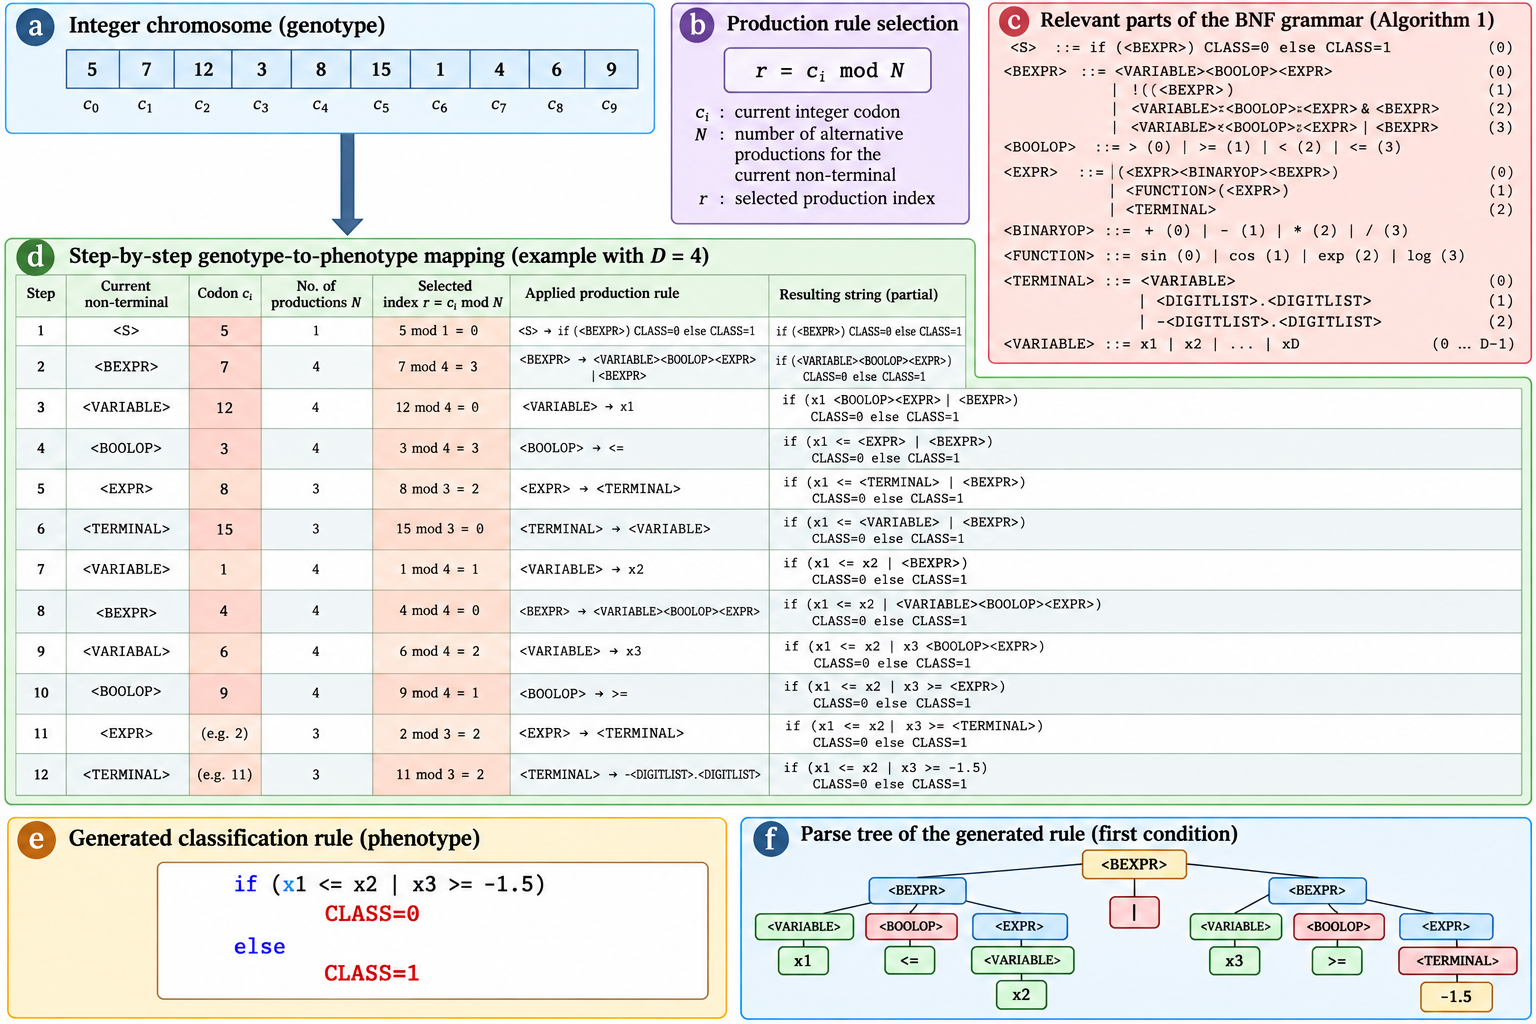
\includegraphics[scale=0.25]{mapping}
\par\end{centering}
\caption{Illustration of the genotype-to-phenotype mapping process employed
by GenClass. Integer-valued codons are sequentially mapped to BNF
production rules using the modulo operation until a complete classification
program is generated.\label{fig:genclass_mapping}}

\end{figure}

The main steps of the algorithm that produces classification programs
are listed subsequently.
\begin{enumerate}
\item \textbf{Initialization step}.
\begin{enumerate}
\item \textbf{Initialize} the Genetic Algorithm parameters: $N_{c}$, the
population size (number of chromosomes); $N_{g}$, the maximum number
of generations; $p_{s}$, the selection rate; and $p_{m}$, the mutation
rate.
\item \textbf{Generate }the initial population of $N_{c}$ chromosomes,
$g_{i},\;i=1,\ldots,N_{c}$, where each chromosome consists of a sequence
of randomly generated integer-valued codons.
\item \textbf{Set} $k=0$, the generation counter.
\end{enumerate}
\item \textbf{Fitness calculation step}.
\begin{enumerate}
\item \textbf{For} $i=1,\ldots,N_{c}$ \textbf{do}
\begin{enumerate}
\item \textbf{Map} each chromosome $g_{i}$ to its corresponding classification
program$C_{i}$ through the genotype-to-phenotype mapping process
defined by the BNF grammar presented in Algorithm \ref{alg:genclass_bnf}.
\item \textbf{Evaluate} the generated classification program $C_{i}$ on
the training set and compute its classification error. The resulting
error value, denoted by $f_{i}$, is used as the fitness value of
the corresponding chromosome $g_{i}$. 
\end{enumerate}
\item \textbf{End For}
\end{enumerate}
\item \textbf{Application of genetic operations}.
\begin{enumerate}
\item \textbf{Selection}: Rank the chromosomes according to their fitness
values in ascending order. The $(1-p_{s})N_{c}$ chromosomes with
the lowest fitness values are directly transferred to the next generation
without modification, while the remaining $p_{s}N_{c}$ chromosomes
are replaced by new offspring generated through the crossover and
mutation operators.
\item \textbf{Crossover}: Generate pairs of offspring by applying the one-point
crossover operator. For each pair of offspring, denoted as $O_{1}$
and $O_{2}$, two parent chromosomes, $P_{1}$ and $P_{2}$, are selected
from the current population using tournament selection. A crossover
point is then randomly selected along the chromosomes, and the genetic
material located after this point is exchanged between the two parents.
Consequently, $O_{1}$ inherits the first part of $P_{1}$ and the
second part of $P_{2}$, whereas $O_{2}$ inherits the first part
of $P_{2}$ and the second part of $P_{1}$. A graphical illustration
of the one-point crossover operation is provided in Figure \ref{fig:onePoint}.
\item \textbf{Mutation}: For each gene$g_{i,j}$ of chromosome $g_{i}$,
a random number $r\in[0,1]$ is generated. If $r\leq p_{m}$, where
$p_{m}$ denotes the mutation rate, the corresponding gene is replaced
by a randomly generated integer value within the predefined range
of admissible codon values. Otherwise, the gene remains unchanged.
\end{enumerate}
\item \textbf{Termination check step}.
\begin{enumerate}
\item \textbf{Set} $k=k+1$
\item \textbf{If} $k\le N_{g}$ \textbf{then go to} Fitness Calculation
step \textbf{else} terminate.
\end{enumerate}
\end{enumerate}
\begin{figure}[H]
\begin{centering}
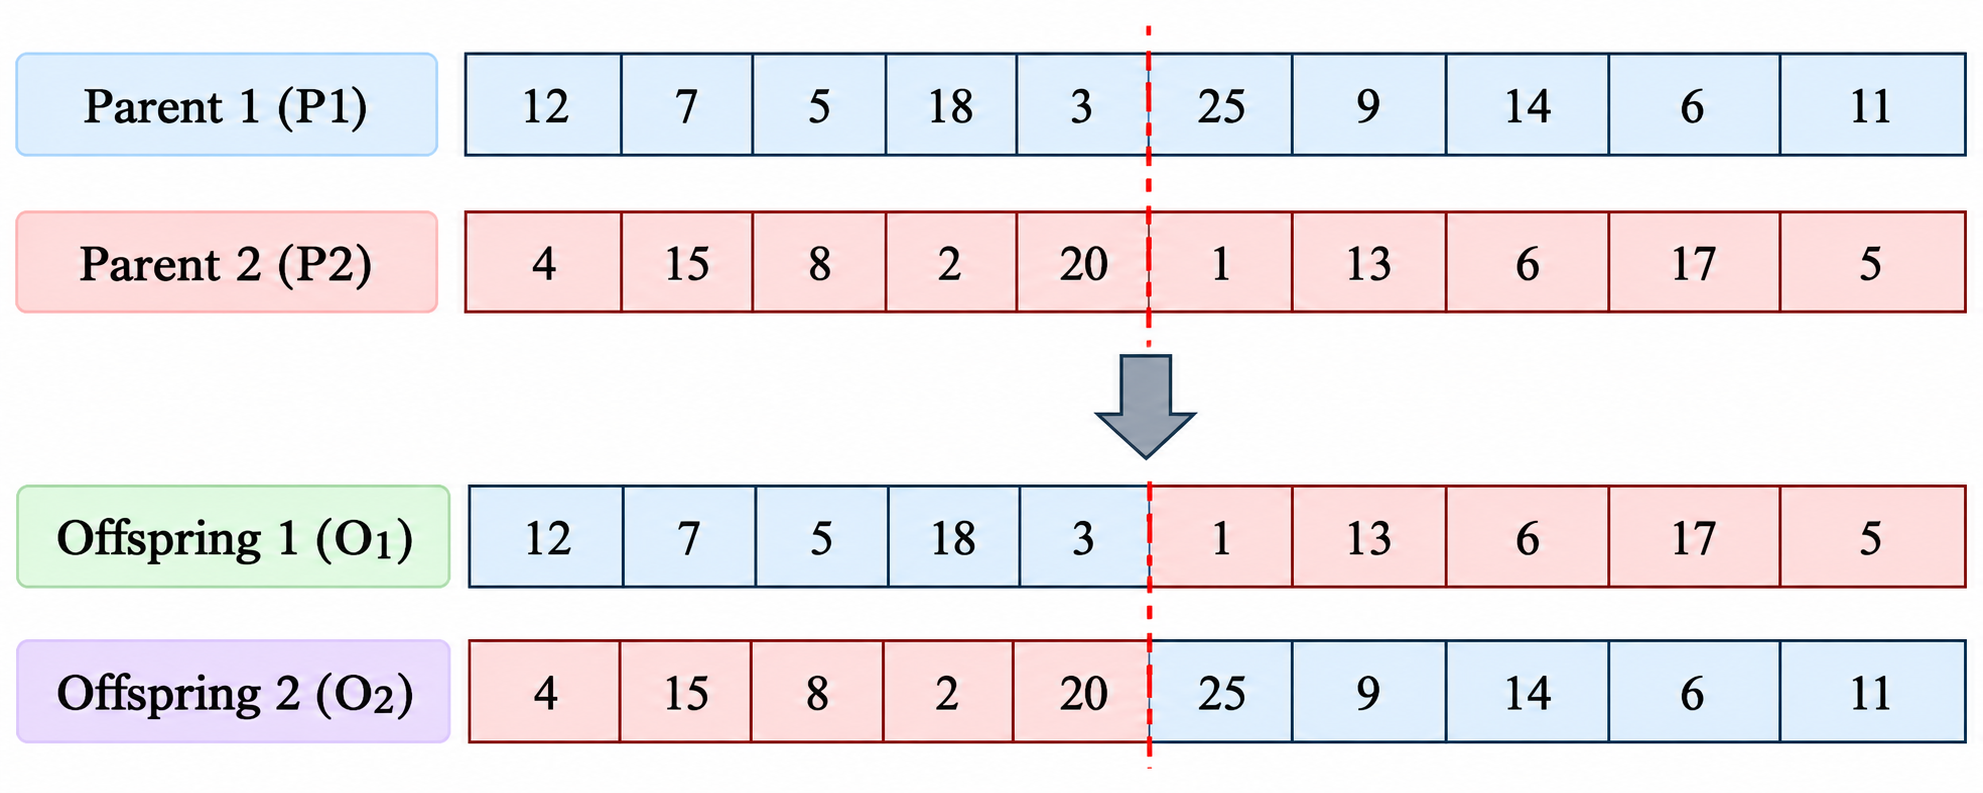
\includegraphics[scale=0.15]{onepoint}
\par\end{centering}
\caption{An example of the one - point crossover method.\label{fig:onePoint}}

\end{figure}


\subsection{The proposed crossover methods}

In the present work, additional crossover techniques are introduced
with the aim of improving the performance of GenClass and enhancing
its ability to escape from local minima of the classification error
function. These crossover operations are applied at each generation
of the evolutionary process to a subset of the current population.
More specifically, a number of chromosomes are randomly selected from
the population and genetic material from each selected chromosome
is exchanged with that of another randomly selected chromosome. In
this way, new combinations of genetic material are introduced into
the population, potentially increasing population diversity and allowing
the evolutionary search to explore previously unvisited regions of
the search space. The number of chromosomes subjected to these additional
crossover operations at each generation is denoted by$\ensuremath{N_{K}}$throughout
the remainder of this work.

The proposed procedure is incorporated into the evolutionary algorithm
described in subsection \ref{subsec:The-rule-construction} and is
executed at each generation after the standard genetic operators of
selection, crossover, and mutation have been applied. In this way,
the additional crossover mechanism operates as an enhancement of the
original evolutionary process without modifying its basic structure.

The proposed crossover techniques, denoted throughout this work as
Standard, Targeted, and TargetedWorst, differ in the strategy employed
to select and exchange genetic material between chromosomes. A detailed
description of each technique is provided in the following subsections.

\subsubsection{The Standard crossover method }

In the Standard crossover technique, for each of the $N_{K}$ selected
chromosomes, denoted by $g_{c}$, a subset of $k$ chromosomes is
randomly selected from the current population,

\[
S=\{g_{r_{1}},g_{r_{2}},\ldots,g_{r_{k}}\}.
\]

The chromosome $\ensuremath{g_{c}}$ is then successively combined
with each chromosome $\ensuremath{g_{r_{i}}},\ensuremath{i=1,\ldots,k}$,
using one-point crossover. For each pair $(g_{c},g_{r_{i}})$, a crossover
point is randomly selected and the corresponding genetic material
is exchanged to produce a candidate offspring chromosome $g_{\mathrm{new}}$.
The fitness of $g_{\mathrm{new}}$ is subsequently evaluated using
its classification error on the training set. If $g_{\mathrm{new}}$
achieves a lower fitness value than the current $g_{c}$, it replaces
$g_{c}$; otherwise, the current chromosome remains unchanged. Importantly,
whenever such an improvement occurs, the updated chromosome becomes
the new $g_{c}$ and is used in the subsequent crossover operation
with $g_{r_{i+1}}$. Therefore, the procedure performs a sequential
improvement of $g_{c}$, allowing beneficial genetic material obtained
from successive crossover operations to be accumulated. After all
$k$ chromosomes in $S$ have been examined, the final improved version
of $g_{c}$ is retained in the population.

The complete procedure of the Standard crossover technique is summarized
in Algorithm \ref{alg:standard_crossover}. The method follows a greedy
acceptance strategy, since a newly generated chromosome replaces the
current chromosome only when it achieves a lower classification error.
Furthermore, each accepted chromosome is immediately used in the subsequent
crossover operation, allowing improvements obtained during successive
crossover trials to be accumulated.

\begin{algorithm}[H]
\caption{Standard crossover technique}
\label{alg:standard_crossover}
\begin{algorithmic}[1]

\Require Population $G=\{g_1,g_2,\ldots,g_{N_c}\}$,
         number of selected chromosomes $N_K$,
         number of crossover trials $k$
\Ensure Updated population $G$

\State Randomly select $N_K$ chromosomes from $G$

\For{each selected chromosome $g_c$}

    \State Randomly select a subset
    $S=\{g_{r_1},g_{r_2},\ldots,g_{r_k}\}$ from $G$

    \For{$i=1$ to $k$}

        \State Randomly select a one-point crossover position

        \State Generate $g_{\mathrm{new}}$ by applying one-point crossover
        between $g_c$ and $g_{r_i}$

        \State Evaluate the fitness $f(g_{\mathrm{new}})$

        \If{$f(g_{\mathrm{new}}) < f(g_c)$}
            \State $g_c \gets g_{\mathrm{new}}$
        \EndIf

    \EndFor

\EndFor

\State \Return $G$

\end{algorithmic}
\end{algorithm}

\subsubsection{The Targeted crossover method }

In the Targeted crossover technique, the exchange of genetic material
is guided by information collected during the genotype-to-phenotype
mapping process. More specifically, the mapping procedure records
the positions of the active codons of each chromosome together with
their semantic role in the generated classification program. These
codons may correspond to different grammatical components, such as
functions, binary operators, Boolean operators, variables, and constants.

For each selected chromosome $g_{c}$, the Targeted technique performs
$k$ crossover trials. At each trial, an active codon position is
randomly selected as the target of the crossover operation. A donor
chromosome $g_{r}$ is then randomly selected from the best fraction
$\rho$ of the current population, and the recorded mapping information
is used to identify an active codon in $g_{r}$ having the same semantic
type as the selected codon of $g_{c}$. Instead of performing an unrestricted
one-point crossover, the Targeted technique transfers a bounded block
of genetic material between the corresponding positions. The size
of this block is determined from the distances to the next active
codons in the two chromosomes and is additionally restricted by a
predefined maximum block size $B_{\max}$. In this way, the transferred
genetic material is associated with similar grammatical components
of the classification programs represented by the two chromosomes.

The resulting chromosome $g_{\mathrm{new}}$ is subsequently mapped
to its corresponding classification program and its fitness is evaluated
on the training set. If

\[
f\left(g_{\mathrm{new}}\right)<f\left(g_{c}\right),
\]

the new chromosome replaces $g_{c}$; otherwise, the current chromosome
remains unchanged. As in the Standard technique, an accepted improvement
is immediately retained and the updated chromosome is used in subsequent
crossover trials. The main difference from Standard crossover is therefore
that the exchange of genetic material is not determined exclusively
by randomly selected crossover points. Instead, information obtained
during the mapping process is exploited to perform crossover between
semantically related regions of the participating chromosomes. This
targeted exchange is intended to increase the probability of producing
meaningful modifications to the generated classification programs
while preserving useful genetic structures already discovered during
the evolutionary process. The complete procedure of the Targeted crossover
technique is summarized in Algorithm \ref{alg:targeted_crossover}.

\begin{algorithm}[Η]
\caption{Targeted crossover technique}
\label{alg:targeted_crossover}
\begin{algorithmic}[1]

\Require Population $G=\{g_1,g_2,\ldots,g_{N_c}\}$,
         number of selected chromosomes $N_K$,
         number of crossover trials $k$,
         elite fraction $\rho$,
         maximum block size $B_{\max}$
\Ensure Updated population $G$

\State Randomly select $N_K$ chromosomes from $G$
\State $N_e \gets \max(2,\lfloor \rho N_c \rfloor)$

\For{each selected chromosome $g_c$}

    \For{$i=1$ to $k$}

        \State Obtain the codon trace of the current chromosome $g_c$

        \State Construct the set $A_c$ of active semantic codons
        corresponding to functions, binary operators,
        Boolean operators, variables, and constants

        \If{$A_c$ is empty}
            \State \textbf{break}
        \EndIf

        \State Randomly select a target codon $a_c \in A_c$
        \State Let $t_c$ be the semantic type of $a_c$

        \State Randomly select a donor chromosome $g_r$
        from the best $N_e$ chromosomes, with $g_r \neq g_c$

        \State Obtain the codon trace of $g_r$

        \State Construct the set $A_r$ of active codons in $g_r$
        having semantic type $t_c$

        \If{$A_r$ is empty}
            \State \textbf{continue}
        \EndIf

        \State Randomly select a compatible donor codon $a_r \in A_r$

        \State Determine $L_c$, the distance from $a_c$
        to the next active codon in $g_c$

        \State Determine $L_r$, the distance from $a_r$
        to the next active codon in $g_r$

        \State $L \gets \min(L_c,L_r,B_{\max})$

        \State Create $g_{\mathrm{new}} \gets g_c$

        \State Copy $L$ codons from $g_r$, starting at $a_r$,
        to the corresponding block of $g_{\mathrm{new}}$
        starting at $a_c$

        \State Evaluate the fitness $f(g_{\mathrm{new}})$

        \If{$f(g_{\mathrm{new}}) < f(g_c)$}
            \State $g_c \gets g_{\mathrm{new}}$
        \EndIf

    \EndFor

\EndFor

\State \Return $G$

\end{algorithmic}
\end{algorithm}

\subsubsection{The TargetedWorst crossover method}

\section{Results\label{sec:Results}}

\subsection{Experimental datasets }

The datasets used in the conducted experiments were downloaded from
the following following online databases:
\begin{enumerate}
\item The UCI website, \url{https://archive.ics.uci.edu/}(accessed on 24
June 2026)\citep{uci}
\item The Keel website, \url{https://sci2s.ugr.es/keel/datasets.php}(accessed
on 24 June 2026)\citep{Keel}.
\end{enumerate}
The used datasets are the following:
\begin{enumerate}
\item \textbf{Alcohol}. This dataset is related to experiments on alcohol
consumption \citep{alcohol}. 
\item \textbf{Appendictis} a dataset originated in \citep{appendicitis}. 
\item Beed.
\item \textbf{Dermatology} dataset \citep{dermatology}, a dataset that
contains measurements for dermatological deceases. 
\item Gene.
\item \textbf{Hayes-roth} dataset \citep{hayes-roth}, a dataset with 3
classes. An artificial data set created to test the behaviour of prototype-based
classifiers. The hobby attribute was generated at random, thus it
is employed to add noise to the data. 
\item \textbf{Hepatitis} dataset. This data set contains a mixture of integer
and real valued attributes, with information about patients affected
by the Hepatitis disease. 
\item \textbf{Housevotes}, that uses data from the Congressional voting
in USA \citep{housevotes}.
\item \textbf{Ionosphere}, that used data from various measurements in the
ionosphere \citep{ion1,ion2}.
\item \textbf{Lymography} \citep{lymography}, which is a dataset with four
distinct classes.
\item \textbf{Nursery} dataset \citep{nursery}. This database was derived
from a hierarchical decision model originally developed to rank applications
for nursery schools. It was used during several years in 1980\textbackslash 's
when there was excessive enrollment to these schools in Ljubljana,
Slovenia, and the rejected applications frequently needed an objective
explanation. The task is to rank applications for a given nursery
school. 
\item The \textbf{Optdigits} dataset \citep{optdigits}, used for the recognition
of handwritten digits from optical scans.
\item Penbased dataset. A digit data base made by collecting 250 samples
from 44 writers, using only (x, y) coordinate information represented
as constant length feature vectors, which were resampled to 8 points
per digit (therefore the data set contains 8 points x 2 coordinates
= 16 attributes). The class label represents the code of the digit
written.
\item \textbf{Phoneme}, where the purpose of this dataset is to distinguish
between nasal and oral sounds.
\item \textbf{PirVision} dataset \citep{pirvision}, that contains occupancy
detection data.
\item \textbf{Satimage} dataset, related to satellite images.
\item \textbf{Segment} dataset \citep{segment}, which is used for image
processing .
\item \textbf{Shuttle} dataset. This data set was generated originally to
extract comprehensible rules for determining the conditions under
which an autolanding would be preferable to manual control of a spacecraft. 
\item \textbf{Spambase}, a dataset used for the detection of spam emails. 
\item \textbf{Spiral}, which is an artificial dataset.
\item \textbf{Student}, a dataset related to some experiments in schools
\citep{student}.
\item \textbf{Splice} dataset, which is inspired by biology.
\item \textbf{Texture} dataset. The aim in this data set is to distinguish
between 11 different textures (Grass lawn, Pressed calf leather, Handmade
paper, Raffia looped to a high pile, Cotton canvas, ...), each pattern
(pixel) being characterised by 40 attributes built by the estimation
of fourth order modified moments in four orientations: 0, 45, 90 and
135 degrees. 
\item \textbf{Thyroid} dataset. This data set is one of the several databases
about Thyroid avalaible at the UCI repository. The task is to detect
is a given patient is normal (1) or suffers from hyperthyroidism (2)
or hypothyroidism (3).
\item \textbf{Twonorm} dataset. This is a 20 dimensional, 2 class classification
problem. Each class is drawn from a multivariate normal distribution.
\item \textbf{Vehicle} dataset. The purpose is to classify a given silhouette
as one of four types of vehicle, using a set of features extracted
from the silhouette. The vehicle may be viewed from one of many different
angles. 
\item \textbf{Yeast} dataset. This database contains information about a
set of Yeast cells. The task is to determine the localization site
of each cell among 10 possible alternatives. 
\item \textbf{EEG} dataset, which is a medical dataset related to EEG measurements\citep{eeg1,eeg2}.
From the original dataset the following cases were obtained: Z\_F\_S,
ZO\_NF\_S, Z\_O\_N\_F\_S and ZONF\_S.
\end{enumerate}
\begin{table}[H]
\caption{The main characteristics of each dataset.\label{tab:The-main-characteristics}}

\centering{}%
\begin{tabular}{|c|c|c|}
\hline 
DATASET & PATTERNS & CLASSES\tabularnewline
\hline 
\hline 
ALCOHOL & 476 & 4\tabularnewline
\hline 
APPENDICITIS & 106 & 2\tabularnewline
\hline 
BEED & 8000 & 4\tabularnewline
\hline 
DERMATOLOGY & 358 & 6\tabularnewline
\hline 
GENE & 3175 & 3\tabularnewline
\hline 
HAYES ROTH & 160 & 3\tabularnewline
\hline 
HEPATITIS & 80 & 2\tabularnewline
\hline 
HOUSEVOTES & 232 & 2\tabularnewline
\hline 
IONOSPHERE & 351 & 2\tabularnewline
\hline 
LYMOGRAPHY & 148 & 4\tabularnewline
\hline 
NURSERY & 12690 & 5\tabularnewline
\hline 
OPTDIGITS & 5620 & 10\tabularnewline
\hline 
PENBASED & 10992 & 10\tabularnewline
\hline 
PHONEME & 5404 & 2\tabularnewline
\hline 
PIRVISION & 15302 & 3\tabularnewline
\hline 
SATIMAGE & 6435 & 7\tabularnewline
\hline 
SEGMENT & 2310 & 7\tabularnewline
\hline 
SHUTTLE & 58000 & 7\tabularnewline
\hline 
SPAMBASE & 4597 & 2\tabularnewline
\hline 
SPIRAL & 2000 & 2\tabularnewline
\hline 
SPLICE & 3190 & 3\tabularnewline
\hline 
STUDENT & 403 & 4\tabularnewline
\hline 
TEXTURE & 5500 & 11\tabularnewline
\hline 
THYROID & 7200 & 3\tabularnewline
\hline 
TWONORM & 7400 & 2\tabularnewline
\hline 
VEHICLE & 846 & 4\tabularnewline
\hline 
YEAST & 1484 & 10\tabularnewline
\hline 
Z\_F\_S & 300 & 3\tabularnewline
\hline 
Z\_O\_N\_F\_S & 500 & 5\tabularnewline
\hline 
ZO\_NF\_S & 500 & 3\tabularnewline
\hline 
ZONF\_S & 500 & 2\tabularnewline
\hline 
\end{tabular}
\end{table}


\subsection{Experimental results }

\begin{table}[H]
\caption{Values for the parameters in experiments.\label{tab:Values-for-the}}

\begin{centering}
\begin{tabular}{|c|c|c|}
\hline 
PARAMETER & MEANING & VALUE\tabularnewline
\hline 
\hline 
$N_{c}$ & Number of chromosomes & 500\tabularnewline
\hline 
$N_{g}$ & Number of allowed generations & 500\tabularnewline
\hline 
$p_{s}$ & Selection rate & 0.9\tabularnewline
\hline 
$p_{m}$ & Mutation rate & 0.05\tabularnewline
\hline 
$N_{K}$ & Crossover items & 10\tabularnewline
\hline 
$H$ & Number of weights for neural networks & 10\tabularnewline
\hline 
\end{tabular}
\par\end{centering}
\end{table}

Table c compares the proposed method (STANDARD) with the original
GenClass method (CLASS) and with the other classifiers over the 31
datasets. All values are classification errors, so lower values indicate
better performance. STANDARD attained the lowest average error, 13.42\%,
followed by CLASS with 16.13\%, while the average errors of the remaining
methods ranged from 33.25\% (GEN) to 44.04\% (NEAT). STANDARD achieved
the lowest error in 23 of the 31 datasets, CLASS in 3, and each of
the other methods in at most 2. Compared with CLASS, the average error
decreases by 2.71 percentage points, a relative reduction of 16.8\%.
Therefore, the new crossover procedure improves the original method
on average, while the improvement over the other methods is considerably
larger.

\begin{table}[H]
\caption{Classification error (\%) of the proposed method (STANDARD) and of
the other classifiers on the 31 datasets. STANDARD is the GenClass
method with the proposed additional crossover procedure, while CLASS
is the original GenClass method without it. The last row (AVERAGE)
reports the mean error over all datasets, and lower values indicate
better performance.\label{tab:methods_comparison}}

\begin{centering}
{\footnotesize{}%
\begin{tabular}{|c|c|c|c|c|c|c|c|c|}
\hline 
{\footnotesize DATASET} & {\footnotesize RBF} & {\footnotesize NEAT} & {\footnotesize DNN} & {\footnotesize ADAM} & {\footnotesize BFGS} & {\footnotesize GEN} & {\footnotesize CLASS} & {\footnotesize STANDARD}\tabularnewline
\hline 
\hline 
{\footnotesize ALCOHOL} & {\footnotesize 49.38\%} & {\footnotesize 66.80\%} & {\footnotesize 39.04\%} & {\footnotesize 57.78\%} & {\footnotesize 41.50\%} & {\footnotesize 39.57\%} & {\footnotesize 16.70\%} & {\footnotesize 11.70\%}\tabularnewline
\hline 
{\footnotesize APPENDICITIS} & {\footnotesize 12.23\%} & {\footnotesize 17.20\%} & {\footnotesize 17.30\%} & {\footnotesize 16.50\%} & {\footnotesize 18.00\%} & {\footnotesize 18.10\%} & {\footnotesize 16.47\%} & {\footnotesize 12.80\%}\tabularnewline
\hline 
{\footnotesize BEED} & {\footnotesize 65.12\%} & {\footnotesize 67.94\%} & {\footnotesize 64.45\%} & {\footnotesize 70.38\%} & {\footnotesize 75.24\%} & {\footnotesize 46.19\%} & {\footnotesize 31.93\%} & {\footnotesize 27.45\%}\tabularnewline
\hline 
{\footnotesize DERMATOLOGY} & {\footnotesize 59.48\%} & {\footnotesize 32.43\%} & {\footnotesize 24.26\%} & {\footnotesize 26.14\%} & {\footnotesize 52.92\%} & {\footnotesize 30.58\%} & {\footnotesize 5.69\%} & {\footnotesize 2.80\%}\tabularnewline
\hline 
{\footnotesize GENE} & {\footnotesize 37.11\%} & {\footnotesize 52.68\%} & {\footnotesize 33.06\%} & {\footnotesize 35.17\%} & {\footnotesize 38.12\%} & {\footnotesize 34.38\%} & {\footnotesize 8.67\%} & {\footnotesize 7.29\%}\tabularnewline
\hline 
{\footnotesize HAYES ROTH} & {\footnotesize 64.36\%} & {\footnotesize 50.15\%} & {\footnotesize 44.65\%} & {\footnotesize 59.70\%} & {\footnotesize 37.33\%} & {\footnotesize 56.18\%} & {\footnotesize 24.31\%} & {\footnotesize 21.08\%}\tabularnewline
\hline 
{\footnotesize HEPATITIS} & {\footnotesize 18.38\%} & {\footnotesize 39.75\%} & {\footnotesize 16.65\%} & {\footnotesize 16.25\%} & {\footnotesize 21.38\%} & {\footnotesize 15.00\%} & {\footnotesize 15.50\%} & {\footnotesize 12.00\%}\tabularnewline
\hline 
{\footnotesize HOUSEVOTES} & {\footnotesize 6.13\%} & {\footnotesize 10.89\%} & {\footnotesize 3.13\%} & {\footnotesize 7.48\%} & {\footnotesize 7.13\%} & {\footnotesize 6.62\%} & {\footnotesize 3.47\%} & {\footnotesize 2.96\%}\tabularnewline
\hline 
{\footnotesize IONOSPHERE} & {\footnotesize 16.22\%} & {\footnotesize 19.67\%} & {\footnotesize 12.57\%} & {\footnotesize 16.64\%} & {\footnotesize 15.29\%} & {\footnotesize 15.14\%} & {\footnotesize 8.10\%} & {\footnotesize 8.74\%}\tabularnewline
\hline 
{\footnotesize LYMOGRAPHY} & {\footnotesize 25.50\%} & {\footnotesize 33.70\%} & {\footnotesize 24.07\%} & {\footnotesize 39.79\%} & {\footnotesize 35.43\%} & {\footnotesize 28.42\%} & {\footnotesize 22.67\%} & {\footnotesize 18.86\%}\tabularnewline
\hline 
{\footnotesize NURSERY} & {\footnotesize 77.10\%} & {\footnotesize 64.11\%} & {\footnotesize 59.73\%} & {\footnotesize 40.94\%} & {\footnotesize 41.40\%} & {\footnotesize 32.14\%} & {\footnotesize 19.65\%} & {\footnotesize 22.27\%}\tabularnewline
\hline 
{\footnotesize OPTDIGITS} & {\footnotesize 71.97\%} & {\footnotesize 72.56\%} & {\footnotesize 64.34\%} & {\footnotesize 72.32\%} & {\footnotesize 67.13\%} & {\footnotesize 67.81\%} & {\footnotesize 27.15\%} & {\footnotesize 14.77\%}\tabularnewline
\hline 
{\footnotesize PENBASED} & {\footnotesize 81.69\%} & {\footnotesize 78.58\%} & {\footnotesize 73.50\%} & {\footnotesize 77.41\%} & {\footnotesize 82.48\%} & {\footnotesize 84.01\%} & {\footnotesize 24.93\%} & {\footnotesize 17.79\%}\tabularnewline
\hline 
{\footnotesize PHONEME} & {\footnotesize 23.32\%} & {\footnotesize 22.43\%} & {\footnotesize 24.34\%} & {\footnotesize 29.43\%} & {\footnotesize 15.58\%} & {\footnotesize 15.55\%} & {\footnotesize 18.89\%} & {\footnotesize 16.82\%}\tabularnewline
\hline 
{\footnotesize PIRVISION} & {\footnotesize 24.58\%} & {\footnotesize 11.84\%} & {\footnotesize 18.28\%} & {\footnotesize 18.38\%} & {\footnotesize 16.94\%} & {\footnotesize 14.31\%} & {\footnotesize 6.53\%} & {\footnotesize 4.38\%}\tabularnewline
\hline 
{\footnotesize SATIMAGE} & {\footnotesize 40.19\%} & {\footnotesize 76.19\%} & {\footnotesize 72.30\%} & {\footnotesize 73.22\%} & {\footnotesize 71.73\%} & {\footnotesize 54.54\%} & {\footnotesize 18.47\%} & {\footnotesize 16.14\%}\tabularnewline
\hline 
{\footnotesize SEGMENT} & {\footnotesize 59.68\%} & {\footnotesize 66.72\%} & {\footnotesize 32.04\%} & {\footnotesize 49.75\%} & {\footnotesize 68.97\%} & {\footnotesize 57.72\%} & {\footnotesize 15.21\%} & {\footnotesize 9.57\%}\tabularnewline
\hline 
{\footnotesize SHUTTLE} & {\footnotesize 32.83\%} & {\footnotesize 29.32\%} & {\footnotesize 2.27\%} & {\footnotesize 21.29\%} & {\footnotesize 42.07\%} & {\footnotesize 20.86\%} & {\footnotesize 1.11\%} & {\footnotesize 1.28\%}\tabularnewline
\hline 
{\footnotesize SPAMBASE} & {\footnotesize 29.35\%} & {\footnotesize 35.77\%} & {\footnotesize 11.30\%} & {\footnotesize 48.05\%} & {\footnotesize 18.16\%} & {\footnotesize 6.37\%} & {\footnotesize 8.97\%} & {\footnotesize 7.28\%}\tabularnewline
\hline 
{\footnotesize SPIRAL} & {\footnotesize 44.87\%} & {\footnotesize 48.66\%} & {\footnotesize 45.24\%} & {\footnotesize 47.67\%} & {\footnotesize 47.99\%} & {\footnotesize 48.66\%} & {\footnotesize 35.65\%} & {\footnotesize 31.25\%}\tabularnewline
\hline 
{\footnotesize SPLICE} & {\footnotesize 40.27\%} & {\footnotesize 55.54\%} & {\footnotesize 48.18\%} & {\footnotesize 75.93\%} & {\footnotesize 30.64\%} & {\footnotesize 30.97\%} & {\footnotesize 7.68\%} & {\footnotesize 7.62\%}\tabularnewline
\hline 
{\footnotesize STUDENT} & {\footnotesize 5.49\%} & {\footnotesize 10.20\%} & {\footnotesize 6.93\%} & {\footnotesize 5.13\%} & {\footnotesize 7.14\%} & {\footnotesize 5.61\%} & {\footnotesize 6.86\%} & {\footnotesize 5.72\%}\tabularnewline
\hline 
{\footnotesize TEXTURE} & {\footnotesize 74.52\%} & {\footnotesize 70.82\%} & {\footnotesize 70.78\%} & {\footnotesize 56.33\%} & {\footnotesize 59.25\%} & {\footnotesize 54.00\%} & {\footnotesize 20.01\%} & {\footnotesize 10.71\%}\tabularnewline
\hline 
{\footnotesize THYROID} & {\footnotesize 10.62\%} & {\footnotesize 18.06\%} & {\footnotesize 7.42\%} & {\footnotesize 3.43\%} & {\footnotesize 5.18\%} & {\footnotesize 7.65\%} & {\footnotesize 1.24\%} & {\footnotesize 0.83\%}\tabularnewline
\hline 
{\footnotesize TWONORM} & {\footnotesize 2.18\%} & {\footnotesize 13.54\%} & {\footnotesize 2.16\%} & {\footnotesize 5.58\%} & {\footnotesize 9.22\%} & {\footnotesize 9.59\%} & {\footnotesize 6.77\%} & {\footnotesize 6.57\%}\tabularnewline
\hline 
{\footnotesize VEHICLE} & {\footnotesize 78.06\%} & {\footnotesize 64.05\%} & {\footnotesize 59.22\%} & {\footnotesize 74.41\%} & {\footnotesize 72.99\%} & {\footnotesize 60.24\%} & {\footnotesize 36.55\%} & {\footnotesize 35.83\%}\tabularnewline
\hline 
{\footnotesize YEAST} & {\footnotesize 67.14\%} & {\footnotesize 71.09\%} & {\footnotesize 68.87\%} & {\footnotesize 57.69\%} & {\footnotesize 77.28\%} & {\footnotesize 69.13\%} & {\footnotesize 45.95\%} & {\footnotesize 44.35\%}\tabularnewline
\hline 
{\footnotesize Z\_F\_S} & {\footnotesize 13.16\%} & {\footnotesize 38.41\%} & {\footnotesize 9.27\%} & {\footnotesize 47.81\%} & {\footnotesize 39.37\%} & {\footnotesize 10.73\%} & {\footnotesize 7.39\%} & {\footnotesize 6.00\%}\tabularnewline
\hline 
{\footnotesize Z\_O\_N\_F\_S} & {\footnotesize 48.70\%} & {\footnotesize 77.08\%} & {\footnotesize 67.80\%} & {\footnotesize 78.79\%} & {\footnotesize 65.67\%} & {\footnotesize 64.81\%} & {\footnotesize 30.32\%} & {\footnotesize 25.32\%}\tabularnewline
\hline 
{\footnotesize ZO\_NF\_S} & {\footnotesize 9.02\%} & {\footnotesize 43.75\%} & {\footnotesize 8.50\%} & {\footnotesize 47.43\%} & {\footnotesize 43.04\%} & {\footnotesize 21.54\%} & {\footnotesize 5.03\%} & {\footnotesize 3.69\%}\tabularnewline
\hline 
{\footnotesize ZONF\_S} & {\footnotesize 4.03\%} & {\footnotesize 5.44\%} & {\footnotesize 2.52\%} & {\footnotesize 11.99\%} & {\footnotesize 15.62\%} & {\footnotesize 4.36\%} & {\footnotesize 2.04\%} & {\footnotesize 2.00\%}\tabularnewline
\hline 
{\footnotesize\textbf{AVERAGE}} & {\footnotesize\textbf{38.47\%}} & {\footnotesize\textbf{44.04\%}} & {\footnotesize\textbf{33.37\%}} & {\footnotesize\textbf{41.57\%}} & {\footnotesize\textbf{40.01\%}} & {\footnotesize\textbf{33.25\%}} & {\footnotesize\textbf{16.13\%}} & {\footnotesize\textbf{13.42\%}}\tabularnewline
\hline 
\end{tabular}}{\footnotesize\par}
\par\end{centering}
\end{table}

The statistical analysis of Table \ref{tab:methods_comparison} is
summarized in Figure \ref{fig:standart_vs_others}. The Friedman test
rejects the hypothesis that all eight methods perform equally ($\chi^{2}(7)=121.47$,
$p=3.8\times10^{-23}$), a result confirmed by the Iman-Davenport
correction ($F(7,210)=38.15$, $p=3.3\times10^{-34}$), with a substantial
effect size (Kendall's $W=0.56$). STANDARD obtains the best mean
rank (1.42), followed by CLASS (2.29), while all the other methods
have mean ranks above 4. In the paired comparisons, STANDARD has lower
error than every other method, with Holm-adjusted Wilcoxon signed-rank
p-values between $8.6\times10^{-6}$ and $1.7\times10^{-5}$ and wins
in 28 to 31 of the 31 datasets. The Hodges-Lehmann estimates of the
median paired difference range from approximately 2.4 percentage points
(CLASS) to 30.4 percentage points (NEAT), none of the 95\% confidence
intervals includes zero, and the effect sizes are large ($r\geq0.77$,
where values around 0.5 or above are conventionally considered large).
The comparison with CLASS requires a careful reading. The bars of
the two methods overlap in the mean-rank panel, which means that the
conservative Nemenyi test does not separate them, since the difference
in mean rank (0.87) is smaller than the critical difference (1.89).
The paired Wilcoxon test, which also takes into account the magnitude
of the differences, detects nevertheless a consistent improvement
(28 wins and 3 losses). STANDARD is worse than CLASS only in three
datasets (IONOSPHERE, NURSERY and SHUTTLE).

\begin{figure}[H]
\begin{centering}
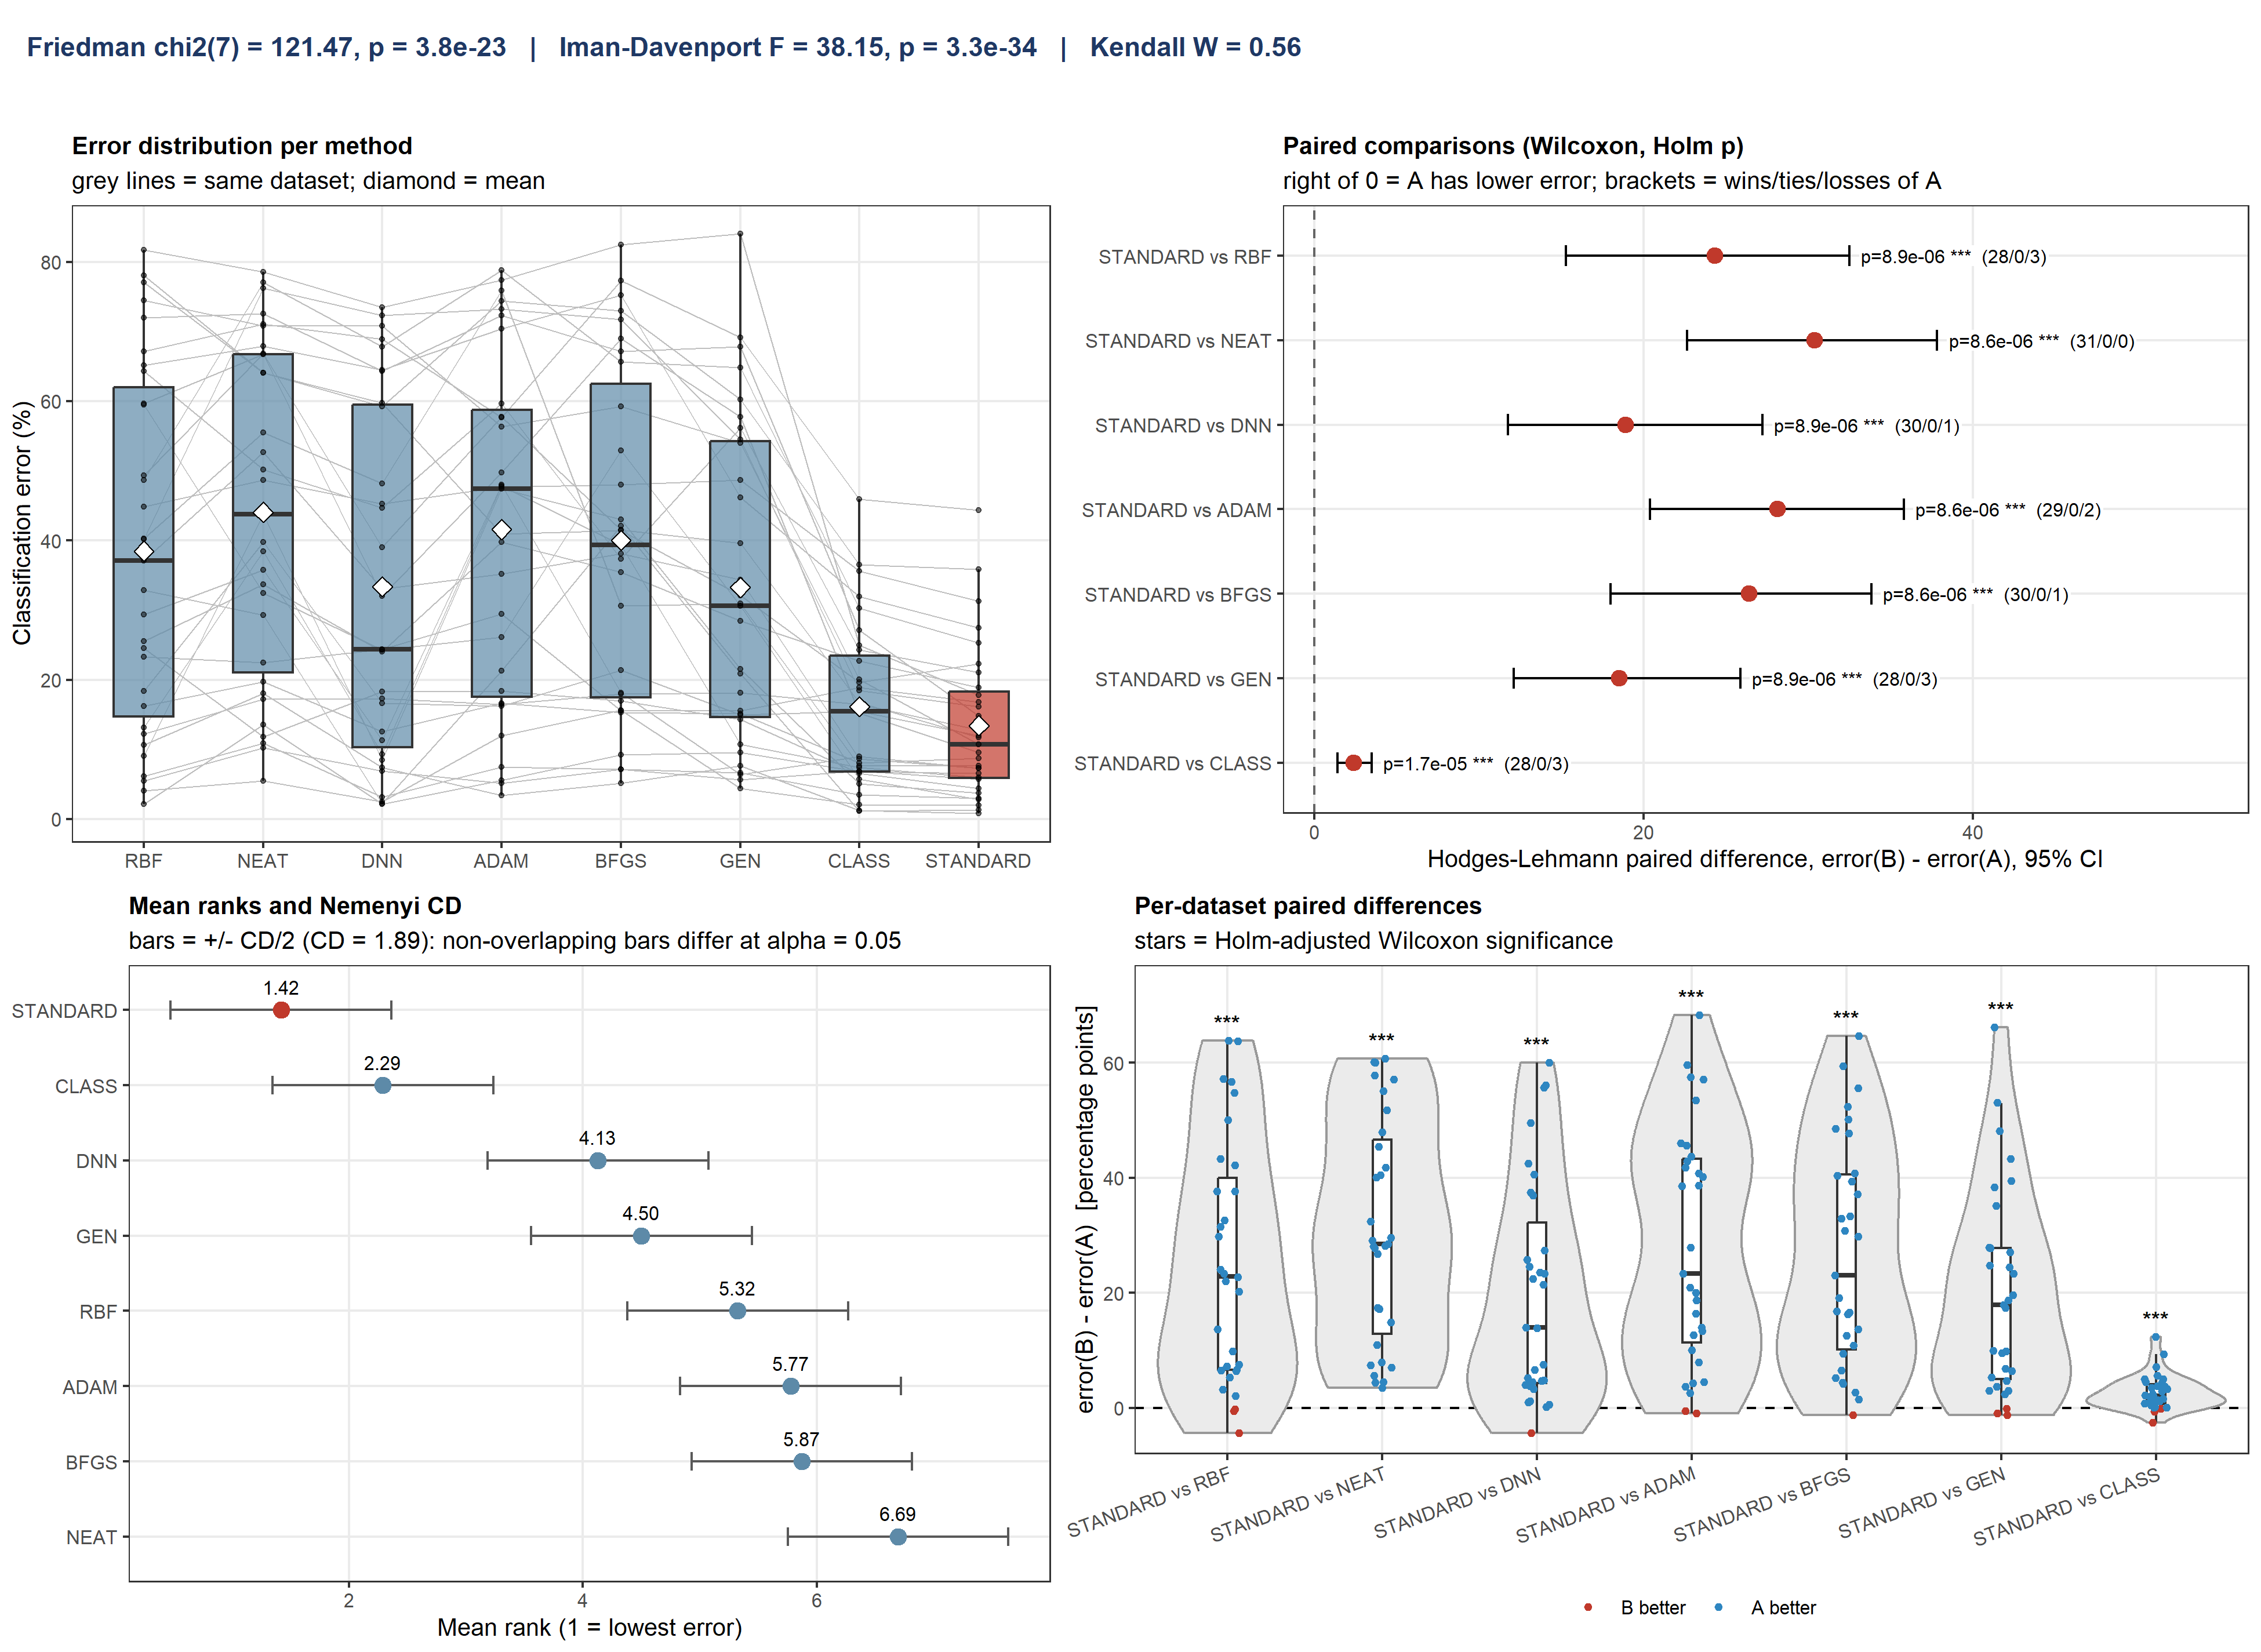
\includegraphics[scale=0.43]{tbl3_summary}
\par\end{centering}
\caption{Statistical comparison of the proposed method (STANDARD) against the
other classifiers over 31 datasets.\label{fig:standart_vs_others}}
\end{figure}

Note: \textit{Box plots: box = interquartile range, thick line = median,
whiskers = $1.5\times IQR$, diamond = mean, dots = datasets, grey
lines join the same dataset. Forest plots: Hodges-Lehmann median paired
difference in error, error(B) \textminus{} error(A), with 95\% CI;
right of the dashed line, A has lower error; labels give the Holm-adjusted
Wilcoxon p-value and the wins/ties/losses of A. Rank panels: mean
Friedman rank (1 = best) $\pm$ CD/2 (Nemenyi); non-overlapping bars
differ at $\alpha$ = 0.05. Bottom right: per-dataset paired differences
(blue: A better, red: B better) or, for \$N\_K\$, the trend with bootstrap
95\% CI. Stars: {*}{*}{*} p \textless{} 0.001, {*}{*} p \textless{}
0.01, {*} p \textless{} 0.05, ns = not significant.}

\subsection{Crossover methods }

Table \ref{tab:crossover_strategies} isolates the effect of the crossover
strategy. STANDARD, in which the exchanged chromosome regions are
selected purely stochastically, achieves the lowest average error
(13.42\%), whereas the two strategies that exploit information collected
during the evolutionary process are less effective, with 15.08\% for
TARGETED and 15.42\% for TARGETEDWORST. STANDARD obtained the lowest
error in 24 of the 31 datasets, compared with 5 for TARGETED and 3
for TARGETEDWORST (a tie between the two targeted strategies in IONOSPHERE
is counted for both). The average gain of STANDARD is 1.66 percentage
points over TARGETED and 2.0 percentage points over TARGETEDWORST,
which correspond to relative reductions of 11.0\% and 13.0\%, respectively.
The two targeted strategies differ little from each other. Hence,
in these experiments, guiding the exchange of genetic material with
information from the evolutionary process did not improve upon the
purely random exchange.

\begin{table}[H]
\caption{Classification error (\%) of the three crossover strategies.\label{tab:crossover_strategies}}

\centering{}%
\begin{tabular}{|c|c|c|c|}
\hline 
DATASET & STANDARD & TARGETED & TARGETEDWORST\tabularnewline
\hline 
\hline 
ALCOHOL & 11.70\% & 17.65\% & 14.04\%\tabularnewline
\hline 
APPENDICITIS & 12.80\% & 16.40\% & 15.40\%\tabularnewline
\hline 
BEED & 27.45\% & 29.48\% & 31.93\%\tabularnewline
\hline 
DERMATOLOGY & 2.80\% & 6.12\% & 5.14\%\tabularnewline
\hline 
GENE & 7.29\% & 9.05\% & 8.20\%\tabularnewline
\hline 
HAYES ROTH & 21.08\% & 22.00\% & 25.38\%\tabularnewline
\hline 
HEPATITIS & 12.00\% & 16.25\% & 16.25\%\tabularnewline
\hline 
HOUSEVOTES & 2.96\% & 3.72\% & 3.04\%\tabularnewline
\hline 
IONOSPHERE & 8.74\% & 7.77\% & 7.77\%\tabularnewline
\hline 
LYMOGRAPHY & 18.86\% & 25.00\% & 21.86\%\tabularnewline
\hline 
NURSERY & 22.27\% & 21.44\% & 21.02\%\tabularnewline
\hline 
OPTDIGITS & 14.77\% & 19.59\% & 19.88\%\tabularnewline
\hline 
PENBASED & 17.79\% & 15.10\% & 23.85\%\tabularnewline
\hline 
PHONEME & 16.82\% & 17.86\% & 17.86\%\tabularnewline
\hline 
PIRVISION & 4.38\% & 4.47\% & 6.53\%\tabularnewline
\hline 
SATIMAGE & 16.14\% & 17.52\% & 18.14\%\tabularnewline
\hline 
SEGMENT & 9.57\% & 12.86\% & 11.26\%\tabularnewline
\hline 
SHUTTLE & 1.28\% & 1.35\% & 0.94\%\tabularnewline
\hline 
SPAMBASE & 7.28\% & 8.22\% & 8.10\%\tabularnewline
\hline 
SPIRAL & 31.25\% & 35.30\% & 34.83\%\tabularnewline
\hline 
SPLICE & 7.62\% & 8.12\% & 8.15\%\tabularnewline
\hline 
STUDENT & 5.72\% & 5.92\% & 6.45\%\tabularnewline
\hline 
TEXTURE & 10.71\% & 17.23\% & 16.59\%\tabularnewline
\hline 
THYROID & 0.83\% & 1.35\% & 1.53\%\tabularnewline
\hline 
TWONORM & 6.57\% & 3.90\% & 5.00\%\tabularnewline
\hline 
VEHICLE & 35.83\% & 39.64\% & 37.03\%\tabularnewline
\hline 
YEAST & 44.35\% & 45.22\% & 47.77\%\tabularnewline
\hline 
Z\_F\_S & 6.00\% & 6.40\% & 7.33\%\tabularnewline
\hline 
Z\_O\_N\_F\_S & 25.32\% & 28.12\% & 30.66\%\tabularnewline
\hline 
ZO\_NF\_S & 3.69\% & 3.08\% & 4.04\%\tabularnewline
\hline 
ZONF\_S & 2.00\% & 1.28\% & 2.04\%\tabularnewline
\hline 
\textbf{AVERAGE} & \textbf{13.42\%} & \textbf{15.08\%} & \textbf{15.42\%}\tabularnewline
\hline 
\end{tabular}
\end{table}

Figure \ref{tab:crossover_strategies} presents the statistical analysis
of Table \ref{tab:crossover_strategies}. The Friedman test indicates
significant differences among the three strategies ($\chi^{2}(2)=22.13$,
$p=1.6\times10^{-5}$, Iman-Davenport $F(2,60)=16.65$, $p=1.8\times10^{-6}$),
with a moderate effect size ($W=0.36$). STANDARD has the best mean
rank (1.32), against 2.27 for TARGETED and 2.40 for TARGETEDWORST.
Since the critical difference is 0.60, the bar of STANDARD does not
overlap with those of the other two strategies, while the bars of
TARGETED and TARGETEDWORST overlap. The paired tests agree with this
picture. STANDARD is significantly better than TARGETED (25 wins and
6 losses, median difference 1.62 percentage points, 95\% CI $[0.58,2.55]$,
$p=0.0018$, $r=0.60$) and than TARGETEDWORST (27 wins and 4 losses,
median difference 1.93 percentage points, 95\% CI $[1.08,2.80]$,
$p=1.6\times10^{-4}$, $r=0.73$). On the contrary, TARGETED and TARGETEDWORST
cannot be distinguished (15 wins, 3 ties and 13 losses, median difference
approximately 0.1 percentage points, 95\% CI $[-0.48,0.95]$, $p=0.64$,
$r=0.09$).

\begin{figure}[H]
\begin{centering}
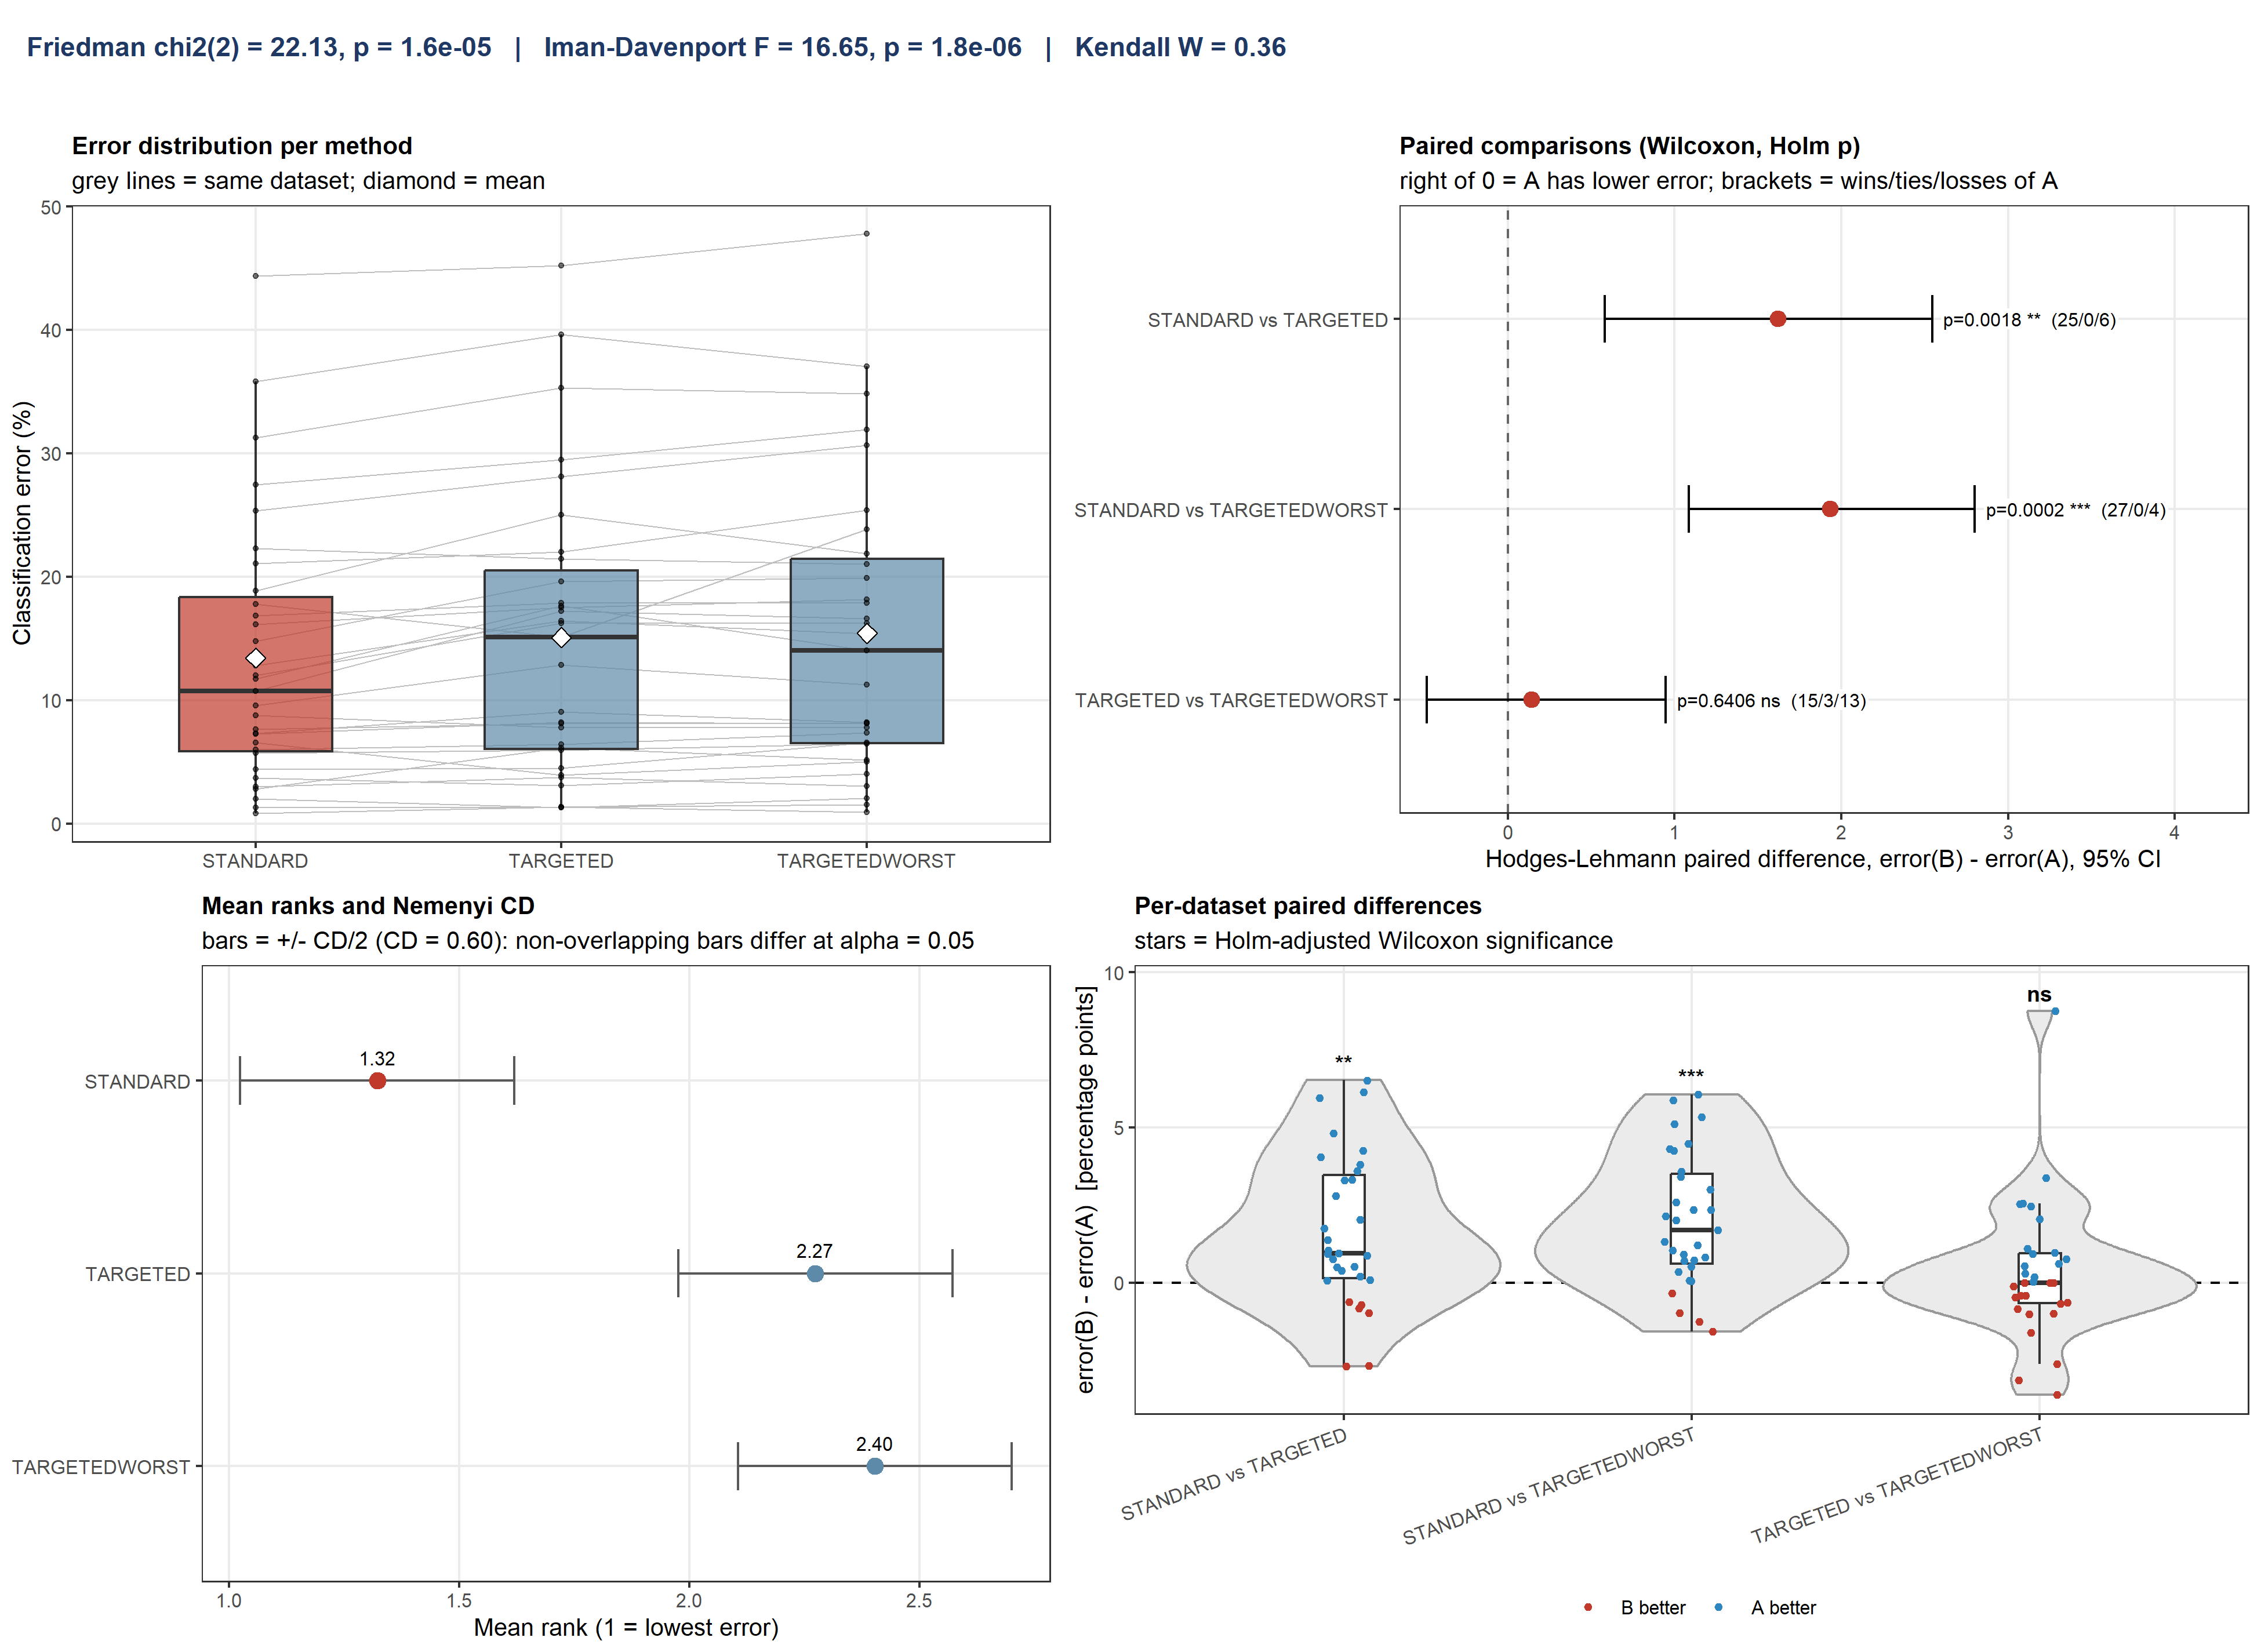
\includegraphics[scale=0.43]{tbl4_summary}
\par\end{centering}
\caption{Statistical comparison of the three \label{fig:crossover_strategies}
(STANDARD, TARGETED, TARGETEDWORST).}
\end{figure}


\subsection{Number of crossing items}

Table \ref{tab:diff_NK} reports the results of the proposed method
when $N_{K}$=2, 5, 10 and 15 chromosomes participate in the crossover.
The column $N_{K}$=10 corresponds to the default value of Table \ref{tab:Values-for-the}
and coincides with the STANDARD column of Table \ref{tab:crossover_strategies}.
The average error decreases monotonically as $N_{K}$ increases, from
14.58\% for $N_{K}$=2 to 13.66\% for $N_{K}$=5, 13.42\% for $N_{K}$=10
and 13.19\% for $N_{K}$=15. The setting $N_{K}$=15 gave the lowest
error in 17 of the 31 datasets, $N_{K}$=5 and $N_{K}$=10 in 7 datasets
each, and $N_{K}$=2 in none. Increasing $N_{K}$ from 2 to 15 reduces
the average error by 1.39 percentage points, whereas each of the two
further increases beyond $N_{K}$=5 changes it by less than 0.3 percentage
points.

\begin{table}[H]
\caption{Experiments with the number that participate in the crossover procedure.\label{tab:diff_NK}}

\centering{}%
\begin{tabular}{|c|c|c|c|c|}
\hline 
DATASET & $N_{K}=2$ & $N_{k}=5$ & $N_{K}=10$ & $N_{K}=15$\tabularnewline
\hline 
\hline 
ALCOHOL & 12.55\% & 13.19\% & 11.70\% & 15.11\%\tabularnewline
\hline 
APPENDICITIS & 15.60\% & 14.40\% & 12.80\% & 15.80\%\tabularnewline
\hline 
BEED & 27.30\% & 26.78\% & 27.45\% & 25.47\%\tabularnewline
\hline 
DERMATOLOGY & 4.74\% & 4.86\% & 2.80\% & 4.00\%\tabularnewline
\hline 
GENE & 8.39\% & 7.29\% & 7.29\% & 6.91\%\tabularnewline
\hline 
HAYES ROTH & 20.77\% & 19.54\% & 21.08\% & 21.39\%\tabularnewline
\hline 
HEPATITIS & 14.00\% & 11.50\% & 12.00\% & 10.00\%\tabularnewline
\hline 
HOUSEVOTES & 3.63\% & 2.78\% & 2.96\% & 3.28\%\tabularnewline
\hline 
IONOSPHERE & 7.60\% & 7.31\% & 8.74\% & 8.80\%\tabularnewline
\hline 
LYMOGRAPHY & 23.71\% & 23.00\% & 18.86\% & 20.57\%\tabularnewline
\hline 
NURSERY & 20.33\% & 22.16\% & 22.27\% & 18.76\%\tabularnewline
\hline 
OPTDIGITS & 17.16\% & 14.56\% & 14.77\% & 13.99\%\tabularnewline
\hline 
PENBASED & 19.95\% & 16.54\% & 17.79\% & 14.22\%\tabularnewline
\hline 
PHONEME & 16.99\% & 16.21\% & 16.82\% & 16.00\%\tabularnewline
\hline 
PIRVISION & 8.49\% & 6.33\% & 4.38\% & 5.35\%\tabularnewline
\hline 
SATIMAGE & 15.91\% & 15.04\% & 16.14\% & 14.93\%\tabularnewline
\hline 
SEGMENT & 11.95\% & 9.91\% & 9.57\% & 9.44\%\tabularnewline
\hline 
SHUTTLE & 1.15\% & 0.62\% & 1.28\% & 0.24\%\tabularnewline
\hline 
SPAMBASE & 7.70\% & 7.98\% & 7.28\% & 7.33\%\tabularnewline
\hline 
SPIRAL & 36.80\% & 33.55\% & 31.25\% & 30.35\%\tabularnewline
\hline 
SPLICE & 7.46\% & 7.18\% & 7.62\% & 7.34\%\tabularnewline
\hline 
STUDENT & 6.11\% & 4.92\% & 5.72\% & 6.70\%\tabularnewline
\hline 
TEXTURE & 12.87\% & 12.73\% & 10.71\% & 12.44\%\tabularnewline
\hline 
THYROID & 1.57\% & 1.06\% & 0.83\% & 0.76\%\tabularnewline
\hline 
TWONORM & 5.62\% & 5.31\% & 6.57\% & 8.01\%\tabularnewline
\hline 
VEHICLE & 37.62\% & 34.81\% & 35.83\% & 33.69\%\tabularnewline
\hline 
YEAST & 46.21\% & 45.69\% & 44.35\% & 44.01\%\tabularnewline
\hline 
Z\_F\_S & 7.00\% & 6.47\% & 6.00\% & 5.67\%\tabularnewline
\hline 
Z\_O\_N\_F\_S & 27.28\% & 27.00\% & 25.32\% & 23.80\%\tabularnewline
\hline 
ZO\_NF\_S & 3.68\% & 3.32\% & 3.69\% & 3.40\%\tabularnewline
\hline 
ZONF\_S & 1.96\% & 1.44\% & 2.00\% & 1.16\%\tabularnewline
\hline 
\textbf{AVERAGE} & \textbf{14.58\%} & \textbf{13.66\%} & \textbf{13.42\%} & \textbf{13.19\%}\tabularnewline
\hline 
\end{tabular}
\end{table}

Figure \ref{fig:effect_of_NK} presents the corresponding statistical
analysis. The Friedman test detects significant differences among
the four settings ($\chi^{2}(3)=21.97$, $p=6.6\times10^{-5}$, Iman-Davenport
$F(3,90)=9.28$, $p=2.1\times10^{-5}$), although with a smaller effect
size than in the previous comparisons ($W=0.24$). The mean rank is
the worst for $N_{K}=2$ (3.35) and the best for $N_{K}=15$ (1.87),
with $N_{K}=5$ (2.27) and $N_{K}=10$ (2.50) in between. The one-sided
Page trend test, which examines whether the error decreases as $N_{K}$
increases, confirms a significant trend ($z=4.08$, $p=2.3\times10^{-5}$).
In agreement, the Spearman correlation between $N_{K}$ and the error
is negative in 23 of the 29 datasets where it is non-zero (median
correlation $-0.6$, sign test $p=0.0023$). The pairwise comparisons
show, however, that this trend is mainly due to the weakness of the
smallest setting. The value $N_{K}=2$ has significantly higher error
than $N_{K}=5$ ($p=3.8\times10^{-4}$), $N_{K}=10$ ($p=0.0047$)
and $N_{K}=15$ ($p=0.0039$), with median differences of approximately
0.8, 1.0 and 1.3 percentage points, respectively. None of the differences
among $N_{K}=5$, 10 and 15 is statistically significant (adjusted$p=0.61$
for 5 versus 10, 0.20 for 5 versus 15 and 0.61 for 10 versus 15),
and their confidence intervals include zero. Therefore, a very small
number of chromosomes in the crossover is detrimental, whereas beyond
$N_{K}=5$ any further benefit is small and is not statistically established
in these experiments, although $N_{K}=15$ has the best mean rank.

\begin{figure}[H]
\begin{centering}
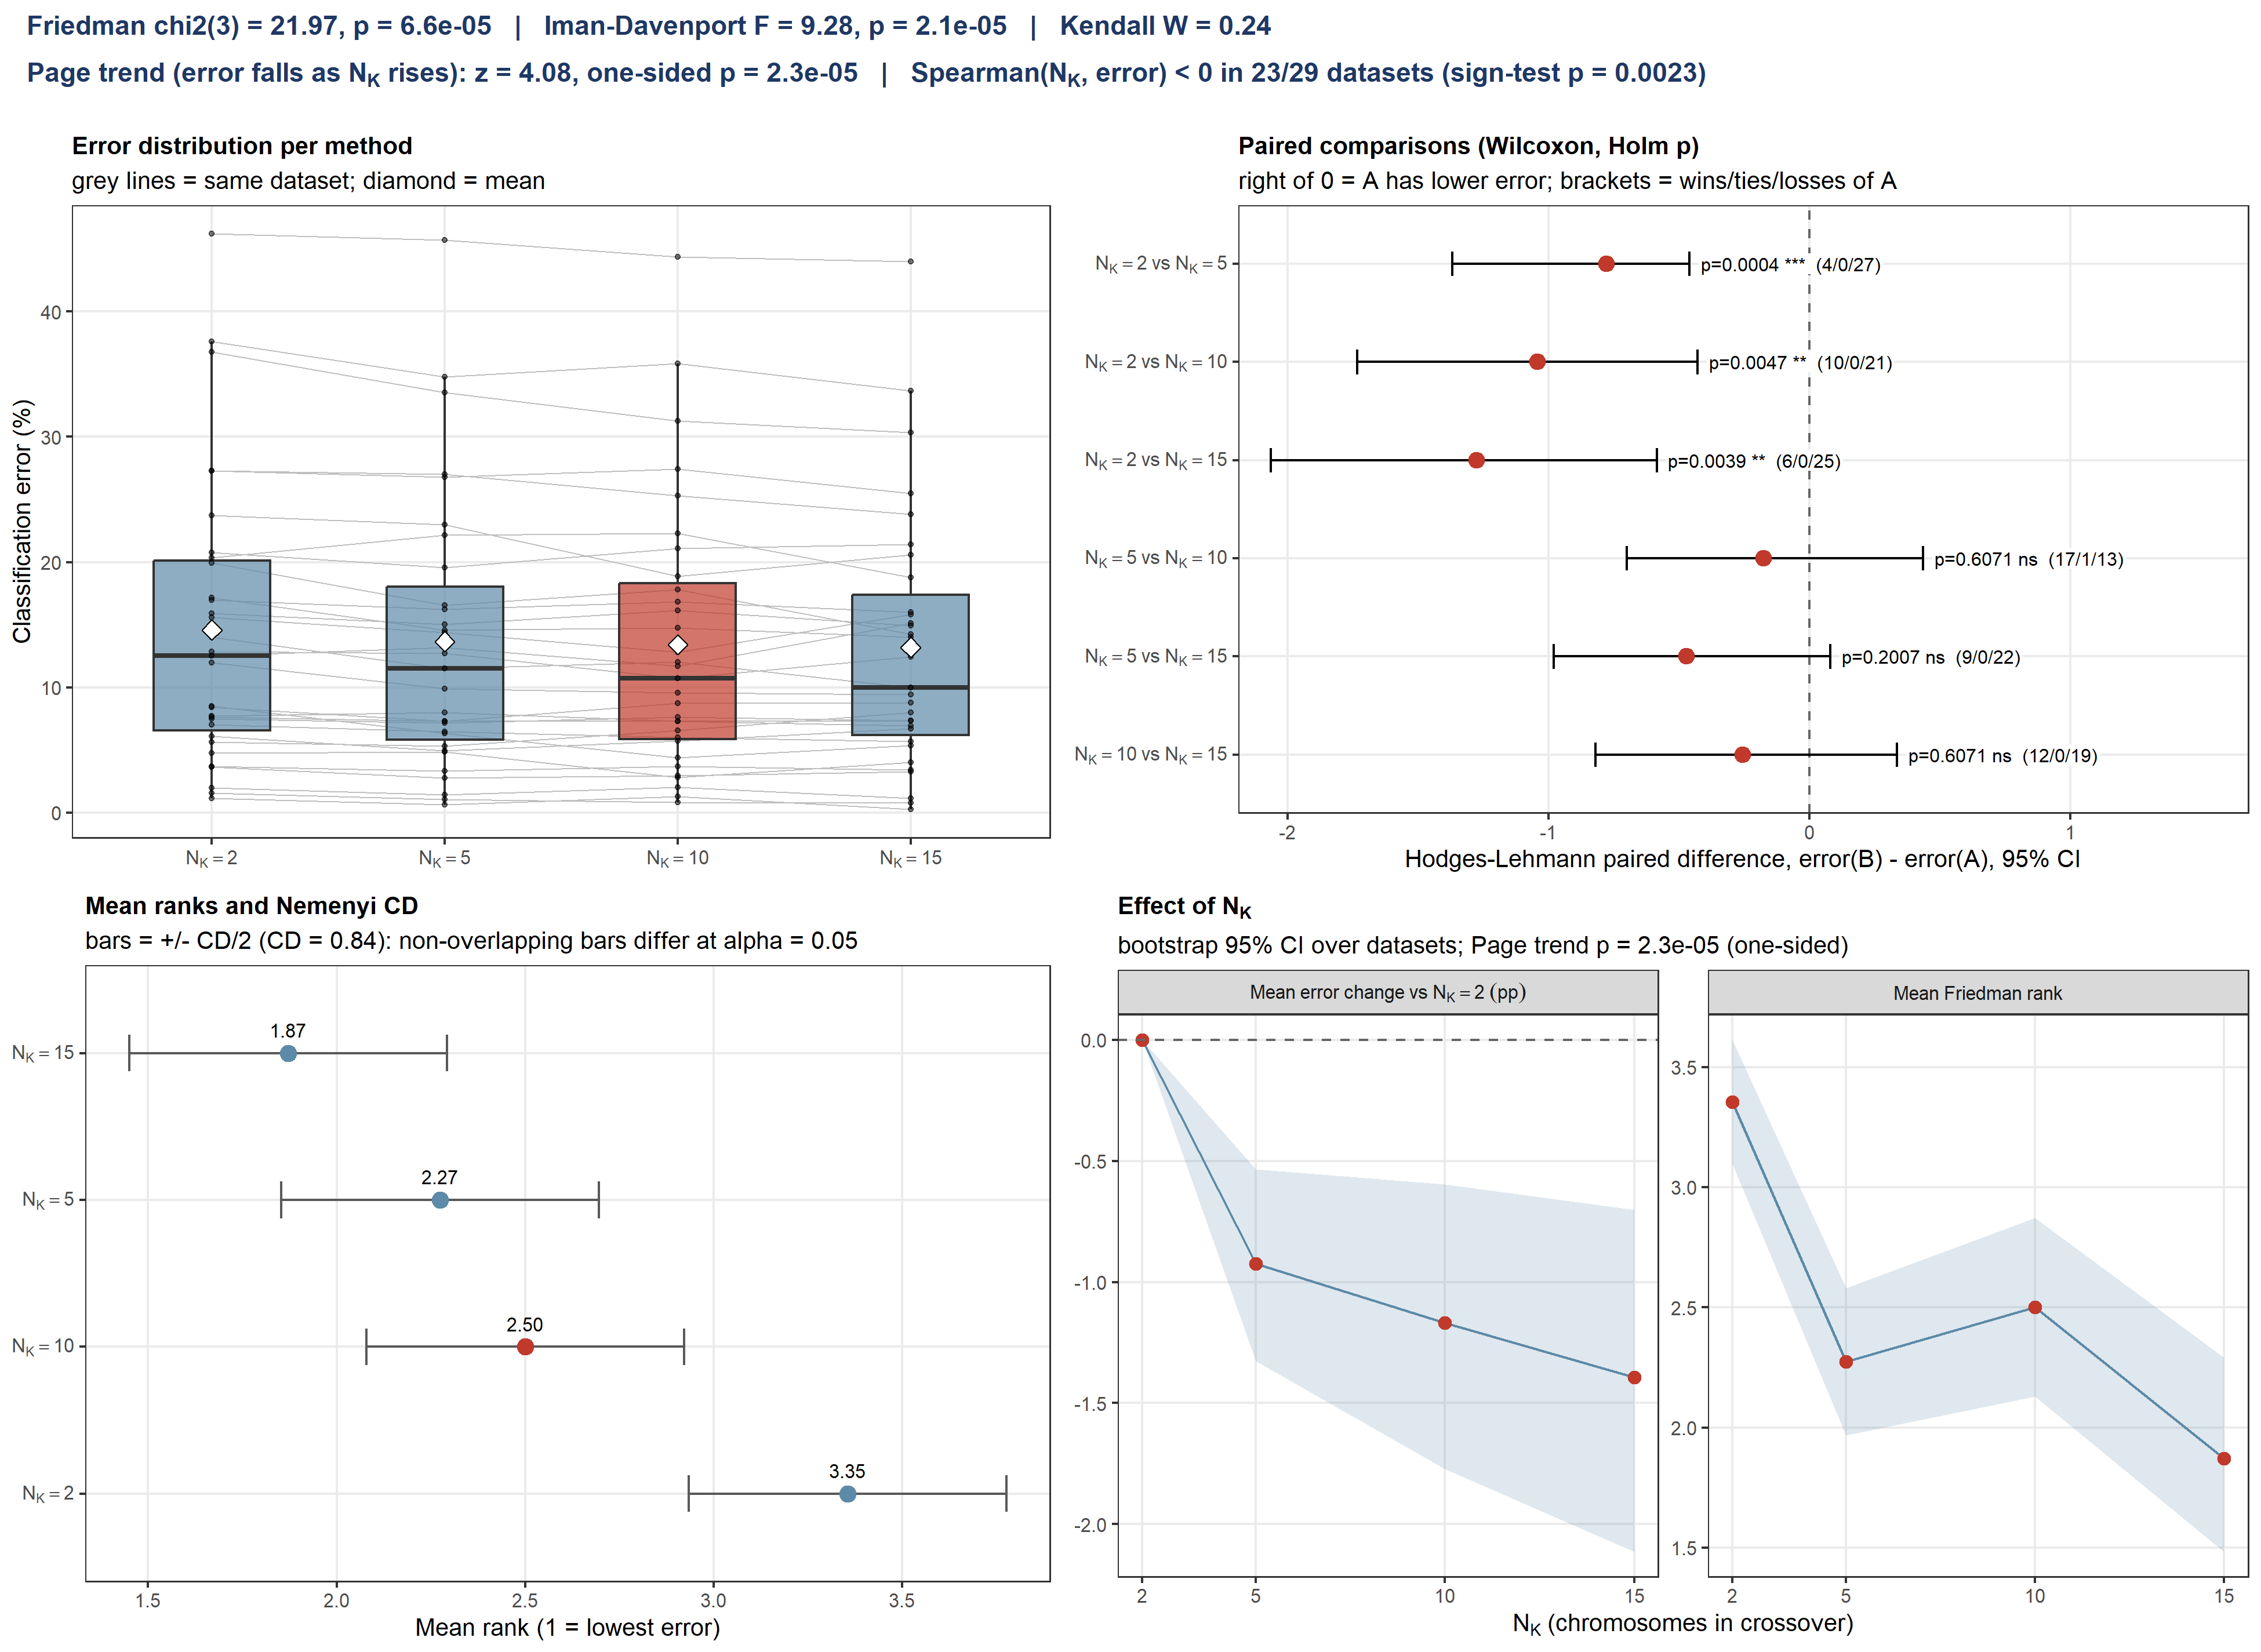
\includegraphics[scale=0.43]{tbl5_summary}
\par\end{centering}
\caption{Effect of the number of chromosomes ($N_{K}$) participating in the
crossover on the proposed method.\label{fig:effect_of_NK}}
\end{figure}


\section{Conclusions\label{sec:Conclusions}}

This work introduced an additional crossover procedure into the GenClass
method, which is applied at every generation to a small number of
randomly selected chromosomes, in order to alleviate the loss of diversity
and the entrapment in local minima of the classification error function.
The procedure was examined in three variants (STANDARD, TARGETED and
TARGETEDWORST) on 31 classification datasets. The STANDARD variant
reduced the average classification error of the original method from
16.13\% to 13.42\%, a relative reduction of 16.8\%, it obtained the
lowest error in 23 of the 31 datasets, and the improvement was statistically
significant, with a considerably larger margin over all the other
classifiers of the comparison.

The experiments also gave a result that differs from what the design
of the targeted variants might suggest. Using information from the
evolutionary process to guide the exchange of genetic material did
not improve on the purely random exchange. STANDARD was significantly
better than both TARGETED and TARGETEDWORST, while the two targeted
variants could not be distinguished from each other. All three variants
obtained a lower average error than the original method (13.42\%,
15.08\% and 15.42\%, against 16.13\%), but statistical significance
was examined only for STANDARD. A possible explanation is that random
exchange preserves more diversity, which is the main weakness of the
original method, but this hypothesis was not tested directly in the
present work.

Finally, the number of chromosomes participating in the crossover
affects the performance, mainly at its lowest values. A very small
number ($N_{K}=2$) was significantly worse than the other settings,
whereas the differences among $N_{K}=5$, 10 and 15 were small and
not statistically significant. A moderate value of $N_{K}$ therefore
seems sufficient. The conclusions are limited to the datasets, the
parameter values and the classification task used in the experiments.

Several directions for future work arise from the present study. First,
the reasons why the targeted variants did not outperform the random
one should be investigated, for example by measuring the diversity
of the population during the evolution, and by designing targeted
operators that preserve diversity or combine random and guided exchanges.
Second, the number of chromosomes participating in the crossover could
be adapted automatically during the evolution instead of being fixed,
and values larger than 15 could be examined, since $N_{K}=15$ had
the best mean rank without a statistically established advantage.
Third, the computational cost of the procedure, which was not measured
here, should be analyzed together with possible parallel implementations.
Finally, the procedure could be evaluated on larger datasets, on other
learning tasks such as regression, and in other methods based on Grammatical
Evolution.

\vspace{6pt}


\authorcontributions{G.G. and I.G.T. conducted the experiments, employing several datasets
and provided the comparative experiments. V.C. a performed the statistical
analysis and prepared the manuscript. All authors have read and agreed
to the published version of the manuscript.}

\funding{This research has been financed by the European Union : Next Generation
EU through the Program Greece 2.0 National Recovery and Resilience
Plan , under the call RESEARCH -- CREATE -- INNOVATE, project name
“iCREW: Intelligent small craft simulator for advanced crew training
using Virtual Reality techniques\textquotedbl{} (project code:TAEDK-06195).}

\institutionalreview{Not applicable.}

\informedconsent{Not applicable.}

\dataavailability{The original contributions presented in this study are included in
the article. Further inquiries can be directed to the corresponding
author. }

\conflictsofinterest{The authors declare no conflicts of interest.}

\begin{adjustwidth}{-\extralength}{0cm}{}

\reftitle{References}
\begin{thebibliography}{999}
\bibitem{holland}J.H. Holland, Genetic algorithms. Scientific american
\textbf{267}, pp. 66-73, 1992.

\bibitem{ec_review}N. Yusup, A. M. Zain, S. Z. M. Hashim, Evolutionary
techniques in optimizing machining parameters: Review and recent applications
(2007--2011), Expert Systems with Applications \textbf{39.10}, pp.
9909-9927, 2012.

\bibitem{gen1}J. Stender, Parallel Genetic Algorithms:Theory \& Applications.
Edition: IOS Press, 1993. 

\bibitem{gen2}D. Goldberg, Genetic Algorithms in Search, Optimization
and Machine Learning, Addison-Wesley Publishing Company, Reading,
Massachussets, 1989.

\bibitem{gen3}Z. Michaelewicz, Genetic Algorithms + Data Structures
= Evolution Programs. Springer - Verlag, Berlin, 1996.

\bibitem{ga_problem1}Y.H. Santana, R.M. Alonso, G.G. Nieto, L. Martens,
W. Joseph, D. Plets, Indoor genetic algorithm-based 5G network planning
using a machine learning model for path loss estimation, Appl. Sci.
\textbf{12}, 3923. 2022.

\bibitem{ga_problem2}X. Liu, D. Jiang, B. Tao, G. Jiang, Y. Sun,
J. Kong, B. Chen, Genetic algorithm-based trajectory optimization
for digital twin robots, Front. Bioeng. Biotechnol \textbf{9}, 793782,
2022.

\bibitem{ga_problem3}K. Nonoyama, Z.Liu, T. Fujiwara, M.M. Alam,
T. Nishi, Energy-efficient robot configuration and motion planning
using genetic algorithm and particle swarm optimization, Energies
\textbf{15}, 2074, 2022.

\bibitem{ga_problem4}K. Liu, B. Deng, Q. Shen, J. Yang, Y. Li, Optimization
based on genetic algorithms on energy conservation potential of a
high speed SI engine fueled with butanol--gasoline blends, Energy
Rep. \textbf{8}, pp. 69--80, 2022.

\bibitem{ga_problem5}G. Zhou, S. Zhu, S. Luo, Location optimization
of electric vehicle charging stations: Based on cost model and genetic
algorithm, Energy \textbf{247}, 123437, 2022.

\bibitem{Doewes}Doewes, R.I.; Nair, R.; Sharma, T. Diagnosis of COVID-19
through blood sample using ensemble genetic algorithms and machine
learning classifier. World J. Eng. 2022, 19, 175--182.

\bibitem{Choudhury} Choudhury, S.; Rana, M.; Chakraborty, A.; Majumder,
S.; Roy, S.; RoyChowdhury, A.; Datta, S. Design of patient specific
basal dental implant using Finite Element method and Artificial Neural
Network technique. J. Eng. Med. 2022, 236, 1375--1387.

\bibitem{Chen} Chen, Q.; Hu, X. Design of intelligent control system
for agricultural greenhouses based on adaptive improved genetic algorithm
for multi-energy supply system. Energy Rep. 2022, 8, 12126--12138.

\bibitem{ge1}M. O’Neill, C. Ryan, Grammatical evolution, IEEE Trans.
Evol. Comput. \textbf{5,}pp. 349--358, 2001.

\bibitem{bnf1}J. W. Backus. The Syntax and Semantics of the Proposed
International Algebraic Language of the Zurich ACM-GAMM Conference.
Proceedings of the International Conference on Information Processing,
UNESCO, 1959, pp.125-132.

\bibitem{ge_program1}C. Ryan, J. Collins, M. O’Neill, Grammatical
evolution: Evolving programs for an arbitrary language. In: Banzhaf,
W., Poli, R., Schoenauer, M., Fogarty, T.C. (eds) Genetic Programming.
EuroGP 1998. Lecture Notes in Computer Science, vol 1391. Springer,
Berlin, Heidelberg, 1998.

\bibitem{ge_program2}M. O’Neill, M., C. Ryan, Evolving Multi-line
Compilable C Programs. In: Poli, R., Nordin, P., Langdon, W.B., Fogarty,
T.C. (eds) Genetic Programming. EuroGP 1999. Lecture Notes in Computer
Science, vol 1598. Springer, Berlin, Heidelberg, 1999.

\bibitem{ge_credit}A. Brabazon, M. O'Neill, Credit classification
using grammatical evolution, Informatica \textbf{30.3}, 2006.

\bibitem{ge_intrusion}S. Şen, J.A. Clark. A grammatical evolution
approach to intrusion detection on mobile ad hoc networks, In: Proceedings
of the second ACM conference on Wireless network security, 2009.

\bibitem{ge_de}I.G. Tsoulos, I.E. Lagaris, Solving differential equations
with genetic programming, Genet Program Evolvable Mach \textbf{7},
pp. 33--54, 2006.

\bibitem{ge_water}L. Chen, C.H. Tan, S.J. Kao, T.S. Wang, Improvement
of remote monitoring on water quality in a subtropical reservoir by
incorporating grammatical evolution with parallel genetic algorithms
into satellite imagery, Water Research \textbf{ 42}, pp. 296-306,
2008.

\bibitem{ge_ant}J. Tavares, F.B. Pereira, Automatic Design of Ant
Algorithms with Grammatical Evolution. In: Moraglio, A., Silva, S.,
Krawiec, K., Machado, P., Cotta, C. (eds) Genetic Programming. EuroGP
2012. Lecture Notes in Computer Science, vol 7244. Springer, Berlin,
Heidelberg, 2012.

\bibitem{ge_trig}C. Ryan, M. O’Neill, J.J. Collins, Grammatical evolution:
Solving trigonometric identities, proceedings of Mendel. Vol. 98.
1998.

\bibitem{ge_music}A.O. Puente, R. S. Alfonso, M. A. Moreno, Automatic
composition of music by means of grammatical evolution, In: APL '02:
Proceedings of the 2002 conference on APL: array processing languages:
lore, problems, and applications July 2002 Pages 148--155. 

\bibitem{ge_nn}Lídio Mauro Limade Campo, R. Célio Limã Oliveira,Mauro
Roisenberg, Optimization of neural networks through grammatical evolution
and a genetic algorithm, Expert Systems with Applications \textbf{56},
pp. 368-384, 2016.

\bibitem{ge_nn2}K. Soltanian, A. Ebnenasir, M. Afsharchi, Modular
Grammatical Evolution for the Generation of Artificial Neural Networks,
Evolutionary Computation \textbf{30}, pp 291--327, 2022.

\bibitem{ge_pacman}E. Galván-López, J.M. Swafford, M. O’Neill, A.
Brabazon, Evolving a Ms. PacMan Controller Using Grammatical Evolution.
In: , et al. Applications of Evolutionary Computation. EvoApplications
2010. Lecture Notes in Computer Science, vol 6024. Springer, Berlin,
Heidelberg, 2010.

\bibitem{ge_supermario}N. Shaker, M. Nicolau, G. N. Yannakakis, J.
Togelius, M. O'Neill, Evolving levels for Super Mario Bros using grammatical
evolution, 2012 IEEE Conference on Computational Intelligence and
Games (CIG), 2012, pp. 304-31.

\bibitem{ge_energy}D. Martínez-Rodríguez, J. M. Colmenar, J. I. Hidalgo,
R.J. Villanueva Micó, S. Salcedo-Sanz, Particle swarm grammatical
evolution for energy demand estimation, Energy Science and Engineering
\textbf{8}, pp. 1068-1079, 2020.

\bibitem{ge_comb}N. R. Sabar, M. Ayob, G. Kendall, R. Qu, Grammatical
Evolution Hyper-Heuristic for Combinatorial Optimization Problems,
IEEE Transactions on Evolutionary Computation \textbf{17}, pp. 840-861,
2013.

\bibitem{ge_crypt}C. Ryan, M. Kshirsagar, G. Vaidya, G. et al. Design
of a cryptographically secure pseudo random number generator with
grammatical evolution. Sci Rep \textbf{12}, 8602, 2022.

\bibitem{ge_decision}P.J. Pereira, P. Cortez, R. Mendes, Multi-objective
Grammatical Evolution of Decision Trees for Mobile Marketing user
conversion prediction, Expert Systems with Applications \textbf{168},
114287, 2021.

\bibitem{ge_analog}F. Castejón, E.J. Carmona, Automatic design of
analog electronic circuits using grammatical evolution, Applied Soft
Computing \textbf{62}, pp. 1003-1018, 2018.

\bibitem{ge_wikipedia}L. Araujo, J. Martinez-Romo, A. Duque, Discovering
taxonomies in Wikipedia by means of grammatical evolution. Soft Comput
\textbf{22}, pp. 2907--2919, 2018. 

\bibitem{ge_trading}C. Martín, D. Quintana, P. Isasi, Grammatical
Evolution-based ensembles for algorithmic trading, Applied Soft Computing
\textbf{84}, 105713, 2019.

\bibitem{ge_bio}Moore, J.H., Sipper, M. (2018). Grammatical Evolution
Strategies for Bioinformatics and Systems Genomics. In: Ryan, C.,
O'Neill, M., Collins, J. (eds) Handbook of Grammatical Evolution.
Springer, Cham. https://doi.org/10.1007/978-3-319-78717-6\_16

\bibitem{ge_glykemia}Hidalgo, J. I., Colmenar, J. M., Risco-Martin,
J. L., Cuesta-Infante, A., Maqueda, E., Botella, M., \& Rubio, J.
A. (2014). Modeling glycemia in humans by means of grammatical evolution.
Applied Soft Computing, 20, 40-53.

\bibitem[(2020)]{genclassMain}Tsoulos, I. G. (2020). Creating classification
rules using grammatical evolution. International Journal of Computational
Intelligence Studies, 9(1-2), 161-171.

\bibitem[(2020)]{genclassSoftx}Anastasopoulos, N.; Tsoulos, I.G.;
Tzallas, A. GenClass: A parallel tool for data classification based
on Grammatical Evolution. SoftwareX 2021, 16, 100830.

\bibitem{genclassPollution}Spyrou, E. D., Stylios, C., \& Tsoulos,
I. (2023). Classification of CO Environmental Parameter for Air Pollution
Monitoring with Grammatical Evolution. Algorithms, 16(6), 300.

\bibitem[(2023)]{genClassNetwork}Margariti, S. V., Tsoulos, I. G.,
Kiousi, E., \& Stergiou, E. (2024). Traffic Classification in Software-Defined
Networking Using Genetic Programming Tools. Future Internet, 16(9),
338.

\bibitem[(1989)]{uci} M. Kelly, R. Longjohn, K. Nottingham, The UCI
Machine Learning Repository, \url{https://archive.ics.uci.edu}.

\bibitem{Keel}J. Alcalá-Fdez, A. Fernandez, J. Luengo, J. Derrac,
S. García, L. Sánchez, F. Herrera. KEEL Data-Mining Software Tool:
Data Set Repository, Integration of Algorithms and Experimental Analysis
Framework. Journal of Multiple-Valued Logic and Soft Computing 17,
pp. 255-287, 2011.

\bibitem[Tzimourta(2018)]{alcohol}Tzimourta, K.D.; Tsoulos, I.; Bilero,
I.T.; Tzallas, A.T.; Tsipouras, M.G.; Giannakeas, N. Direct Assessment
of Alcohol Consumption in Mental State Using Brain Computer Interfaces
and Grammatical Evolution. Inventions 2018, 3, 51.

\bibitem{appendicitis}Weiss, Sholom M. and Kulikowski, Casimir A.,
Computer Systems That Learn: Classification and Prediction Methods
from Statistics, Neural Nets, Machine Learning, and Expert Systems,
Morgan Kaufmann Publishers Inc, 1991.

\bibitem{dermatology}G. Demiroz, H.A. Govenir, N. Ilter, Learning
Differential Diagnosis of Eryhemato-Squamous Diseases using Voting
Feature Intervals, Artificial Intelligence in Medicine. \textbf{13},
pp. 147--165, 1998.

\bibitem[(1977)]{hayes-roth}B. Hayes-Roth, B., F. Hayes-Roth. Concept
learning and the recognition and classification of exemplars. Journal
of Verbal Learning and Verbal Behavior \textbf{16}, pp. 321-338, 1977.

\bibitem[(2002)]{housevotes}R.M. French, N. Chater, Using noise to
compute error surfaces in connectionist networks: a novel means of
reducing catastrophic forgetting, Neural Comput. \textbf{14}, pp.
1755-1769, 2002.

\bibitem[(2004)]{ion1}J.G. Dy , C.E. Brodley, Feature Selection for
Unsupervised Learning, The Journal of Machine Learning Research \textbf{5},
pp 845--889, 2004.

\bibitem{ion2}S. J. Perantonis, V. Virvilis, Input Feature Extraction
for Multilayered Perceptrons Using Supervised Principal Component
Analysis, Neural Processing Letters \textbf{10}, pp 243--252, 1999.

\bibitem[(2002)]{lymography}G. Cestnik, I. Konenenko, I. Bratko,
Assistant-86: A Knowledge-Elicitation Tool for Sophisticated Users.
In: Bratko, I. and Lavrac, N., Eds., Progress in Machine Learning,
Sigma Press, Wilmslow, pp. 31-45, 1987. 

\bibitem{nursery}Olave, M., Rajkovic, V., \& Bohanec, M. (1989).
An application for admission in public school systems. Expert Systems
in Public Administration, 1, 145-160.

\bibitem{optdigits}Kaynak, C. (1995). Methods of combining multiple
classifiers and their applications to handwritten digit recognition.
Unpublished master’s thesis, Bogazici University.

\bibitem[(2023)]{pirvision}Emad-Ud-Din, M., \& Wang, Y. (2023). Promoting
occupancy detection accuracy using on-device lifelong learning. IEEE
Sensors Journal, 23(9), 9595-9606.

\bibitem{segment}M. Dash, H. Liu, P. Scheuermann, K. L. Tan, Fast
hierarchical clustering and its validation, Data \& Knowledge Engineering
\textbf{44}, pp 109--138, 2003.

\bibitem[(2007)]{student}P. Cortez, A. M. Gonçalves Silva, Using
data mining to predict secondary school student performance, In Proceedings
of 5th FUture BUsiness TEChnology Conference (FUBUTEC 2008) (pp. 5--12).
EUROSIS-ETI, 2008.

\bibitem[(2007)]{eeg1}R. G. Andrzejak, K. Lehnertz, F.Mormann, C.
Rieke, P. David, and C. E. Elger, “Indications of nonlinear deterministic
and finite-dimensional structures in time series of brain electrical
activity: dependence on recording region and brain state,” Physical
Review E, vol. 64, no. 6, Article ID 061907, 8 pages, 2001. 

\bibitem{eeg2}A. T. Tzallas, M. G. Tsipouras, and D. I. Fotiadis,
“Automatic Seizure Detection Based on Time-Frequency Analysis and
Artificial Neural Networks,” Computational Intelligence and Neuroscience,
vol. 2007, Article ID 80510, 13 pages, 2007. doi:10.1155/2007/80510

\end{thebibliography}

\end{adjustwidth}{}
\end{document}
